% June 2015 (TOC contents linked in blue in pdf file)
% This template was prepared by Dorothea F. Brosius of the 
% Institute for Electronics and Applied Physics, University of Maryland, College Park, MD
% The template was last updated in June 2015
% Thesis Main Page used with thesis.sty based on the
% University of Maryland Electronic Thesis and Dissertation (ETD) Style Guide (2014)

% The YourInformation file was created by Freja Nordsiek, 2014.
% Code for linking the TOC titles to the text in the pdf file was created by Freja Nordsiek, 2014.

% Modified by Francisco Salces-Carcoba 2018.

% This file contains a number of user defined commands
% used throughout the main file. To add use the notation
% \newcommand{NAME_OF_COMMAND}[NO_OF_ARGS]{COMMAND_ACTION}

%%%%%%%%%%%%%%%%%%%%%%%%%%%%%%%%%%%%%%%%%%%%%%%%%%%%%%%%%%%%%%%%%%%%%%%%
% Select the version that fits how you are making this LaTeX document (its driver).
% The first two are the most likely ones to be needed.

\newcommand{\mydriver}{pdftex}
% \newcommand{\mydriver}{dvipdfmx}
% \newcommand{\mydriver}{dvipdfm} 
% \newcommand{\mydriver}{dvips} 
% \newcommand{\mydriver}{dvipsone} 
% \newcommand{\mydriver}{ps2pdf} 

%%%%%%%%%%%%%%%%%%%%%%%%%%%%%%%%%%%%%%%%%%%%%%%%%%%%%%%%%%%%%%%%%%%%%%%%
% Unit formatter for inline math.
\newcommand{\units}[3]{${#1 #2 \,\rm{#3}}$}

% Used to get a vertical distance after \hline
\newcommand{\tbsp}{\rule{0pt}{18pt}}

 

\documentclass[12pt,\mydriver]{umdthesis-2}

\usepackage{titlesec}
   \titleformat{\chapter}
      {\normalfont\large}{Chapter \thechapter:}{1em}{}

\usepackage{graphicx}
\usepackage{cite}
\usepackage{lscape}
\usepackage{indentfirst}
\usepackage{latexsym}
\usepackage{multirow}
\usepackage{tabls}
\usepackage{wrapfig}
\usepackage{slashbox}
\usepackage{longtable}
\usepackage{supertabular}
\usepackage{subeqn}
\usepackage{subfigure}
\usepackage{setspace}

% The command below works with PcTex. You may have to choose the appropriate driver if dvips does not work.
% \usepackage[dvips, bookmarks, colorlinks=true, plainpages=false, 
%			citecolor=blue, urlcolor=blue, filecolor=blue, 
%			linkcolor=blue]{hyperref}
% This file contains a number of user defined environments
% used throughout the main file. To add use the notation
% \newenvironment{NAME_OF_ENV}{BEFORE}{AFTER}

%%%%%%%%%%%%%%%%%%%%%%%%%%%%%%%%%%%%%%%%%%%%%%%%%%%%%%%%%%%%%%%%%%%%%%%%
\newenvironment{title_env}
	{\setstretch{2}
	 \setlength{\textwidth}{5.9in}
	 \setlength{\textheight}{9in}
	 \setlength{\topmargin}{-.50in}
     %\setlength{\topmargin}{0in} % Use if printer makes top margin 1/2 inch.
	 \setlength{\oddsidemargin}{.55in}
 	 \setlength{\parindent}{.4in}
	 \pagestyle{empty}}
	{\ignorespacesafterend}
%%%%%%%%%%%%%%%%%%%%%%%%%%%%%%%%%%%%%%%%%%%%%%%%%%%%%%%%%%%%%%%%%%%%%%%%
\newenvironment{preface_env}
	{\pagestyle{plain}
 	 \pagenumbering{roman}
	 \setcounter{page}{2}}
	{\ignorespacesafterend}
%%%%%%%%%%%%%%%%%%%%%%%%%%%%%%%%%%%%%%%%%%%%%%%%%%%%%%%%%%%%%%%%%%%%%%%%
\newenvironment{lists_env}
	{\setstretch{1}
	 \small
	 \normalsize}
	{\ignorespacesafterend}
%%%%%%%%%%%%%%%%%%%%%%%%%%%%%%%%%%%%%%%%%%%%%%%%%%%%%%%%%%%%%%%%%%%%%%%%
\newenvironment{chapter_env}
	{\setlength{\parskip}{0em}
	 \setstretch{2}
	 \small\normalsize
	 \setcounter{page}{1}
	 \pagenumbering{arabic}}
	{\ignorespacesafterend}
%%%%%%%%%%%%%%%%%%%%%%%%%%%%%%%%%%%%%%%%%%%%%%%%%%%%%%%%%%%%%%%%%%%%%%%%
\newenvironment{bib_env}
	{\setstretch{1}
	 \small\normalsize}
	{\ignorespacesafterend}
%%
%% macros.tex
%%

% \newcommand{\onlinecite}[1]{\nocite{#1}\citenum{#1}}
% Changes
\def\cs{{\ {\clubsuit}}}

% Length

\def\nm{{\ {\rm nm}}}						% nm
\def\mm{{\ {\rm mm}}}						% mm
\def\cm{{\ {\rm cm}}}						% cm
\def\micron{{\ \mu{\rm m}}}					% Microns
\def\angstrom{{\ \mbox{{\rm \AA}}}}			% Angstroms

% Electrons
\def\tesla{{\ {\rm T}}}						% tesla
\def\nohm{{\ {\rm n}\Omega}}				% nohm
\def\uohm{{\ \mu\Omega}}					% uohm
\def\mohm{{\ {\rm m}\Omega}}				% mohm
\def\ohm{{\ \Omega}}						% ohm
\def\kohm{{\ {\rm k}\Omega}}				% Kohm
\def\Mohm{{\ {\rm M}\Omega}}				% Mohm
\def\conductance#1{{\times{#1}\ \Omega^{-1}}} % Mhos

\def\density#1{{\times{#1}\ {\rm cm}^{-2}}}				% Density
\def\mobility#1{{\times{#1}\ {\rm cm}^{2}/{\rm V s}}} 	% Mobility
\def\microvolt{{\ \mu{\rm V}}}				% Microvolts
\def\volt{{\ {\rm V}}}						% volts

% Current
\def\pA{{\ {\rm pA}}}						% pA
\def\nA{{\ {\rm nA}}}						% nA
\def\uA{{\ \mu{\rm A}}}						% uA
\def\mA{{\ {\rm mA}}}						% mA
\def\amp{{\ {\rm A}}}						% A
\def\kA{{\ {\rm kA}}}						% kA
\def\MA{{\ {\rm MA}}}						% MA
\def\GA{{\ {\rm GA}}}						% GA
\def\TA{{\ {\rm TA}}}						% TA

% Vots
\def\volt{{\ {\rm V}}}						% V
\def\mV{{\ {\rm mV}}}						% mV
\def\uV{{\ \mu{\rm V}}}					% uV
\def\nV{{\ {\rm nV}}}						% nV
\def\pV{{\ {\rm pV}}}						% pV
\def\fV{{\ {\rm fV}}}						% fV

% Energy
\def\eV{{\ {\rm eV}}}						% eV
\def\meV{{\ {\rm meV}}}						% meV
\def\ueV{{\ \mu{\rm eV}}}					% ueV
\def\neV{{\ {\rm neV}}}						% neV

% Frequency
\def\uHz{{\ \mu{\rm Hz}}}					% uHz
\def\mHz{{\ {\rm mHz}}}						% mHz
\def\Hz{{\ {\rm Hz}}}						% Hz
\def\kHz{{\ {\rm kHz}}}						% kHz
\def\MHz{{\ {\rm MHz}}}						% MHz
\def\GHz{{\ {\rm GHz}}}						% GHz
\def\THz{{\ {\rm THz}}}						% THz

% Time
\def\fs{{\ {\rm fs}}}						% fs
\def\ps{{\ {\rm ps}}}						% ps
\def\ns{{\ {\rm ns}}}						% ns
\def\us{{\ \mu{\rm s}}}						% us
\def\ms{{\ {\rm ms}}}						% ms
\def\second{{\ {\rm s}}}					% s

% Temperature
\def\kelvin{{\ {\rm K}}}					% K
\def\mK{{\ {\rm mK}}}						% mK
\def\uK{{\ \mu{\rm K}}}						% uK
\def\nK{{\ {\rm nK}}}						% nK

% mass
\def\kg{{\ {\rm kg}}}					% kg
\def\gram{{\ {\rm g}}}					% g
\def\mg{{\ {\rm mg}}}						% mg
\def\ug{{\ \mu{\rm g}}}						% ug
\def\ng{{\ {\rm ng}}}						% ng


% Magnetic Field
\def\gauss{{\ {\rm G}}}					% T
\def\tesla{{\ {\rm T}}}					% T
\def\mT{{\ {\rm mT}}}						% mT
\def\uT{{\ \mu{\rm T}}}						% uT
\def\nT{{\ {\rm nT}}}						% nT

% AMO abbriviations
\def\Er{{{E_R}}}	
\def\El{{{E_{\rm L}}}}						% Er
\def\kr{{{k_{\rm R}}}}
\def\kl{{{k_{\rm L}}}}								% kr
\def\Rb87{^{87}\rm{Rb}}					% Rb 87
\def\UoverTC{(U/t)_{\rm c}}					% t/U_c

\def\nbar{\left<{\hat n}_k\right>}					% average number
\def\nbarexpt{\left<n(k_x,k_y)\right>}				% average number

% Specific Symbols
\def\DeltaSAS{{\Delta_{{\rm SAS}}}}			% DeltaSAS
\def\HeFour{{^4{\rm He}}}					% Helium 4
\def\HeThree{{^3{\rm He}}}					% Helium 3
\def\lb{{l_B}}								% Magnetic Length
\def\DoverL{{d/\lb}}						% d/l
\def\DoverLcrit{{\DoverL_{\rm crit}}}		% d/l_crit
\def\Bpar{{B_{\|}}}							% B Parallel
\def\Bperp{{B_{\perp}}}						% B Perpindicular
\def\AlGaAs#1#2{{{\rm Al}_{#1}{\rm Ga}_{#2}{\rm As}}} % Al_xGa_{1-x}As
\def\Schrodinger{{Schr\"odinger\ }}

% Basic mathematical symbols
\def\ex{{\mathbf e}_x}                            % e_x
\def\ey{{\mathbf e}_y}                            % e_y
\def\ez{{\mathbf e}_z}                            % e_z
\def\epos{{\mathbf e}_+}                            % e_z
\def\eneg{{\mathbf e}_-}                            % e_z
\def\shorttimes{\!\times\!}                            % e_z
\def\e1{{\mathbf e}_1}                            % e_1
\def\e2{{\mathbf e}_2}                            % e_2
\def\e3{{\mathbf e}_3}                            % e_3
\def\e{{\mathbf e}}                            % e
\def\k{{\mathbf k}}                            % k
\def\x{{\mathbf x}}                            % x
\def\q{{\mathbf q}}                            % x
\mathchardef\Im="023D



\def\shorteq{\! = \!}                            % e_z
\DeclareMathAlphabet\mathbfcal{OMS}{cmsy}{b}{n}

% Operators
\def\fx{\hat{F}_x}  
\def\fy{\hat{F}_y}  
\def\fz{\hat{F}_z}  
\def\fp{\hat{F}_+}  
\def\fm{\hat{F}_-}  

% RF dressed state symbols
\def\Omrf{\Omega_{RF}}
\def\omrf{\omega_{RF}}
\def\xyz{\ket{xyz}}
\def\XYZ{\ket{XYZ}}

%bra/ket commands
\def\bra#1{\mathinner{\langle{#1}|}}
\def\ket#1{\mathinner{|{#1}\rangle}}
\newcommand{\braket}[2]{\langle #1|#2\rangle}
\def\Bra#1{\left<#1\right|} 
\def\Ket#1{\left|#1\right>}
{\catcode`\|=\active
  \gdef\Braket#1{\left<\mathcode`\|"8000\let|\BraVert {#1}\right>}}
\def\BraVert{\egroup\,\mid@vertical\,\bgroup}



% Other useful stuff
\newcommand{\note}[1]{\textcolor{red}{[\textrm{#1}]}} % Make 


%set footnote separation
%onehalfspacing baselineskip looks like double spaced for footnote size text
\singlespacing
\setlength{\footnotesep}{\baselineskip}

%setup the document margins etc.
\doublespacing
\renewcommand{\baselinestretch}{2}
\setlength{\textwidth}{5.9in}
\setlength{\textheight}{9in}
\setlength{\topmargin}{-.50in}
%\setlength{\topmargin}{0in}    %use this setting if the printer makes the the top margin 1/2 inch instead of 1 inch
\setlength{\oddsidemargin}{.55in}
\setlength{\parindent}{.4in}
%\pagestyle{empty}

\begin{document}

	\begin{title_env} 
		% !TEX root = mainthesis.tex
%Abstract Page 

\hbox{\ }

\renewcommand{\baselinestretch}{1}
\small \normalsize

\begin{center}
\large{{ABSTRACT}} 

\vspace{3em} 

\end{center}
\hspace{-.15in}
\begin{tabular}{ll}
Title of dissertation:   
&				      {\large  TOPOLOGICAL DISPERSION RELATIONS IN } \\
&				      {\large  SPIN-ORBIT COUPLED BOSE GASES} \\
\ \\
&                     {\large  Ana Valdés-Curiel,} \\
&					  {\large  Doctor of Philosophy, 2019} \\
\ \\
Dissertation directed by: & {\large  Professor Ian Spielman} \\
&  							{\small	 Joint Quantum Institute,} \\
&  							{\small	 National Institute of Standards and Technology and} \\
&  							{\small	 University of Maryland College Park} \\
\end{tabular}

\vspace{3em}

\renewcommand{\baselinestretch}{2}
\large \normalsize

Quantum degenerate gases have proven to be an ideal platform for the  simulation of complex systems. Due to their high level of control it is possible to readily design and implement systems with effective Hamiltonians in the laboratory. In particular, experimental tools such as optical lattices and light induced gauge fields offer the possibility of creating new atomic `materials' with interaction dominated or topologically non-trivial band structures. This thesis focuses on the development of new tools for the characterization and control of engineered quantum systems, and applies them to create and characterize a topological system with Rashba-type spin-orbit coupling. 

The underlying properties of such engineered systems depend on their single particle energies and it is therefore important to characterize them. I describe a Fourier transform spectroscopy technique to probe the single particle spectrum of a quantum system and apply it to measure the dispersion relation of a spin-1 spin-orbit coupled Bose-Einstein condensate (BEC). Fourier transform spectroscopy relies only on measuring the unitary evolution under a Hamiltonian of interest and can be applied generically to any system with long enough coherent evolution.

Decoherence of quantum systems due to uncontrolled fluctuations of the environment presents fundamental obstacles in quantum science. I describe an implementation of continuous dynamical decoupling (CDD) in a spin-1 BEC. We applied a strong radio-frequency (RF) magnetic field to the ground state hyperfine manifold of Rubidium-87 atoms, generating a dynamically protected dressed system that was first-order insensitive to changes in magnetic field. The CDD states constitute effective clock states and we observed a reduction in sensitivity to magnetic field of up to four orders of magnitude. I show that the CDD states can be coupled in a fully connected way unlike bare atomic states which are constrained by selection rules. 

Finally, I describe the quantum engineering of Rashba-type SOC using Raman coupled CDD states. Our engineered system had non-trivial topology but without an underlying crystalline structure that yields integer Chern numbers in conventional materials. We validated our procedure using Fourier transform spectroscopy to measure the full dispersion relation that contained only a single Dirac point. We measured the quantum geometry underlying the dispersion relation and obtained the topological index using matter-wave interferometry. In contrast to crystalline materials, where topological indices take on integer values, our continuum system reveals an unconventional half-integer Chern number. 

  
		%Titlepage

\thispagestyle{empty}
\hbox{\ }
\vspace{1in}
\renewcommand{\baselinestretch}{1}
\small\normalsize
\begin{center}

\large{{TOPOLOGICAL DISPERSION RELATIONS IN}} \\
\large{{SPIN-ORBIT COUPLED BOSE GASES}}
\ \\
\ \\
\large{by} \\
\ \\
\large{Ana Vald\'es Curiel}%Your full name as it appears in University records.
\ \\
\ \\
\ \\
\ \\
\normalsize
Dissertation submitted to the Faculty of the Graduate School of the \\
University of Maryland, College Park in partial fulfillment \\
of the requirements for the degree of \\
Doctor of Philosophy \\
2019
\end{center}

\vspace{7.5em}

\noindent Advisory Committee: \\
Professor Alicia Kollar, Chair \\
Professor Gretchen Campbell \\
Professor Mohammad Hafezi, Dean's representative \\
Professor Norbert Linke  \\
Professor Trey Porto \\
Professor Ian Spielman, Advisor \\






 
		\include{Copyright}
	\end{title_env}

	\begin{preface_env}
		%Preface

\renewcommand{\baselinestretch}{2}
\small\normalsize
\hbox{\ }
 
\vspace{-.65in}

\begin{center}
\large{Preface} 
\end{center} 

A few weeks after I had started writing this thesis Ian came to me and asked if I had learned all the physics I wish I had known while I was doing my PhD. I felt a bit puzzled. I had been operating the lab, analyzing data and writing papers for a while, of course I already knew the physics relevant to my research! It finally hit me when I was writing the introductory chapters how many subtleties I had missed and how much I still didn't know. As experimental physicists being in the lab can give us some physical intuition and a sense of understanding but sometimes that is not enough. This was a very striking and unexpected side effect of the thesis and I invite experimentalists reading this to challenge their lab intuition. 

In the end, I actually found it very enjoyable to look back at the history of our field and to put my research into a bigger context. I never thought the words thesis and  enjoyable could go well together! My advice for a graduate student starting to write a thesis is try to enjoy the ride, it will definitely be stressful and overwhelming but it is also a great learning opportunity. 

A PhD thesis is not just a service for oneself but also a service to other students and new members of the lab. I had this in mind during the process of writing and I hope that future students find this document helpful. 
 
		\include{Foreword}
		%Dedication

\renewcommand{\baselinestretch}{2}
\small\normalsize
\hbox{\ }
 
\vspace{-.65in}

% 
% \large{Dedication}
% 
\begin{center}
\textit{For my parents and in the} \\
\textit{memory of Dr. Ernesto Valdés Krieg}
\end{center} 
		%Acknowledgments

\renewcommand{\baselinestretch}{2}
\small\normalsize
\hbox{\ }
 
\vspace{-.65in}

\begin{center}
\large{Acknowledgments} 
\end{center} 

\vspace{1ex}

I was very lucky to be surrounded by an amazing group of people throughout my PhD. None of this would have been possible without them and I feel infinitely lucky and grateful for that. 

I would like to start by thanking my advisor Dr. Ian Spielman. 

I was exposed to a cold atoms lab for the first time when I spent a summer working in a lab of Dr. Luis Orozco. I thank him for giving me this opportunity that would later define the course of my PhD. He is a great mentor who cares very deeply about his students. I am extremely grateful for his support throughout my years at UMD, for all the delicious meals and bread, the concerts and the good stories. 

I would like to thank Dr. Bill Phillips for always being  warm and welcoming and for taking the time to participate in `paper torture' sessions with me. I learned a lot of physics (and history of physics) from this interactions. I would also like to thank him for being an endless source of chocolate. 

My research was performed at the RbLi lab at UMD, where I was lucky  that my path crossed with a lot of wonderful physicists and also now good friends. First I would like to thank  Daniel Campbell, Ryan Price and Andika Putra for welcoming me to RbLi and patiently teaching me about the lab. A very special thank you goes to our former postdoc Dimitri Trypogeorgos for taking me under his wing and becoming my lab brother. He is a brilliant scientist who really helped to shape my PhD. I am extremely grateful for all his physics and life teachings as well as his friendship. I would also like to thank and acknowledge my current lab mates. Qi-Yu Liang for her brutal honesty and for the physics discussions that tended to start with confusion and end with enlightenment. I also thank her for the rabbit pictures and videos and for our food discussions. I admire her determination and her ability to stand up for what she believes in. Mingshu Zhao and Junheng Tao for their enthusiasm and diligently taking over the tasks of building a new apparatus. I am also grateful for their encouraging words when I was writing this thesis and my last paper. They are very smart physicists and I am sure there will be great things to come in the new lab. 

Our lab was also very fortunate to have a couple brilliant visitors. I thank Nathan Lundblad for all his help when the lab was feeling a bit understaffed. I would also like to thank Russ `Mr. Broadband' Andersson for all the helpful experimental diagnostics gadgets, the very thorough help on calculations and comments on papers, and for always being in such a good mood. It was great fun to have him around. 

I have been away from the lab many months now and instead spending a great deal of time in my office. I would like to thank my office mates for making it all more fun. Hector Soza Mart\'inez for being absolutely ridiculous. His sense of humor reminds me that we shouldn't take ourselves too seriously. Joao `the champ' Braz for being a great theory buddy. I really enjoyed our physics discussions and am thankful for all the thorough comments on the Rashba paper. I am also thankful that he made me leave my desk to get a beer when he thought I needed a break. Dina Genkina for always listening and offering encouraging words, also for the constant flow of Kit Kats. 

Marcell Gall, Pierre Dussarat, Daniel Ohl de Melo (las visitas)

(los chicos) 

(ihop y extendidos)

Paco, common denominator 

(familia)




	\end{preface_env}
	
	\begin{lists_env}
		\tableofcontents 
		\newpage
		% \listoftables 
		% \newpage
		\listoffigures 
		\newpage
		\addcontentsline{toc}{chapter}{List of Abbreviations}
		%List of Abbreviations

\renewcommand{\baselinestretch}{1}
\small\normalsize
\hbox{\ }

\vspace{-3em}


\begin{center}
\large{List of Abbreviations}
\end{center} 

\vspace{3pt}

\begin{tabular}{ll}
$\alpha$ & alpha \\
$\beta$  & beta \\
&  \\ 
NIST & National Institute of Standards and Technology \\
JQI & Joint Quantum Institute
\end{tabular}

		\newpage
	\end{lists_env}

	\begin{chapter_env}
		% \include{Cheat_sheet}
		% !TEX root = mainthesis.tex
% Informs the editor to look one folder up for the main file.
%Chapter 1

\renewcommand{\thechapter}{1}

\chapter{Introduction}

Bose statistics were first developed in 1924 to describe the quantum behavior of photons \cite{bose_plancks_1924}, quanta of light with integer valued spin. Today, we routinely produce atomic Bose-Einstein condensates in the laboratory and even use them as a platform for the analog simulation of complex systems. The field has certainly come a long way! 

Bose-Einstein condensathion (BEC) in atomic gases was observed for the first time in 1995 in dilute vapors of $\Rb87$~\cite{anderson_observation_1995} and $^{23}$Na~\cite{davis_bose-einstein_1995}. Even though the BEC phase had been predicted for a long time it wasn't until experimental techniques of laser cooling and trapping were developed that bosonic atoms were cooled down to temperatures low enough for condensation to occur\footnote{For a more in depth story of the BEC field I highly recommend reading~\cite{ketterle_w._making_1999}.}. The experimental realization of this new phase of matter opened new possibilities for studying macroscopic quantum phenomena such as superfluidity [xx] and and coherent matter waves [xx] and jump-started an ever growing filed of research. For this achievement Eric Cornell, Carl Wieman and Wolfgang Ketterle were awarded the 2001 Nobel Prize in physics. 

It has been more than 20 years (and many more in the learning of atomic physics) and the field of quantum degenerate gases has expanded to include degenerate Fermi gases and spinor gases. As the field continues to grow, new control and detection techniques are being constantly developed, enabling the use of BECs and ultracold atomic systems in general not just as an object of study by themselves but as tools for a wide range of scientific endeavors, from precision measurements [add citation of clocks and edn]to the analog simulation of complex systems.

Quantum degenerate gases have proven to be an ideal platform for quantum simulation. A very straightforward example is the use of optical lattices where the periodic potential imparted by standing waves of light serve as an analogue to the crystal structure of a solid. Perhaps the first iconic realization of a quantum simulation was the study of the Bose-Hubbard model in three-dimensional optical lattices, the bosonic analogue of a model which is believed to be relevant to high $T_c$ superconductors. 


 creating new exotic atomic `materials', with interaction-dominated or topologically non-trivial band structures that can help deepen our understanding of certain physical phenomena. 



 

This thesis focuses on the development of new tools for the characterization and control of engineered quantum systems, and applies them to create and characterize a system with Rashba-type~\cite{bychkov_oscillatory_1984} spin-orbit coupling. The creation of new `atomic' materials requires the ability to characterize the single particle energies. We developed a  Fourier transform spectroscopy technique which allows us to probe the single particle spectrum of a system, and thereby verifying our quantum engineering, by only looking at quantum coherent evolution. 

Atomic systems are susceptible to environmental noise, leading to undesirable effects such as the loss of coherence. In particular laboratories such as ours greatly suffer from noise in ambient magnetic fields and go through great efforts to diminish its effects. We implemented continuous dynamical decoupling (CDD) on a set of internal atomic states which renders them first order insensitive to changes in magnetic field, effectively turning them into clock-like states. These CDD states are not just a robust basis for performing experiments, they additionally gave us access to new matrix elements which were essential for the engineering of the Rashba Hamiltonian. (Talk about lattice and Hofstater) . 

The simulation of the Rashba Hamiltonian is certainly condensed matter inspired. Spin-orbit coupling can be present in two-dimensional materials and it plays an important role in the quantum spin Hall effect and the realization of topological insulators. The beauty of our system is we can depart from conventional materials, for example, by considering a system with Rashba SOC but without an underlying crystalline structure. We do so in the last part of this thesis and find that our conventional understanding of the topology of Bloch bands is defied. 


\section{Thesis overview}

In Chapters 2 and 3 I will describe the basic theory of Bose-Einstein condensation and the technical details of our experimental apparatus that produces $\Rb87$ BECs. In Chapter 4 I will describe our quantum simulation toolkit, the standard techniques that we use to manipulate and detect ensembles of ultracold atoms that are necessary for all of our experiments. Chapter 5 describes a Fourier transform spectroscopy technique that exploits the relation between quantum coherent evolution and the underlying spectrum of a system and that was used to characterize experiments described later in the thesis. Chapter 6 describes an implementation of continuous dynamical decoupling that helped to both make our system more robust against environmental noise and also allowed us to couple the internal states of the atoms in new ways that were not possible before, opening the path for new kinds of quantum simulations described in Chapters 7 and 8. In Chapter 8 I describe the experimental realization of Rashba spin-orbit coupling for a quantum system without a crystalline structure and has unconventional topology characterized by non-integer topological invariants. Finally, Chapter 8 describes the experimental implementation of a fractional period adiabatic superlattice, an intermediate step necessary for us to generate Hofstadter cylinders with non-zero magnetic flux in the future. 

Apendix are experiments that I contributed to but are not included in the thesis. Also things related to new apparatus?



A great deal of current research focuses on understanding
the physical consequences of these new materials, and
experimental studies of topological insulators and superconductors in solid state systems continue apace. Furthermore,
there is significant activity in exploring the nature of the
strongly correlated phases of matter that arise in these
materials, notably to construct strong-correlation variants of
these topological states of weakly interacting electrons.
Theory suggests many interesting possibilities, which are still
seeking experimental realization and verification.
Such questions are ideally addressed using realizations with
cold atomic gases. Cold atomic gases allow strongly interacting phases of matter to be explored in controlled experimental
settings. However, a prerequisite for quantum simulations of
such issues is the ability to generate topological energy bands
for cold atoms. This poses a significant challenge, even at this
single-particle level. Realizing topological energy bands
typically requires either the introduction of effective orbital
magnetic fields acting on neutral atoms and/or the introduction of a spin-orbit coupling between the internal spin states of
an atom and its center-of-mass motion. This is an area of
research that has attracted significant attention over the last
years, both theoretical and experimental. Much progress has
been made in developing techniques to generate artificial
magnetic fields and spin-orbit coupling for neutral atoms
(Zhai, 2015; Dalibard, 2016; Aidelsburger, Nascimbene, and
Goldman, 2017). The use of these techniques in the setting of
optical lattices has led to the realization and characterization
of topological Bloch bands for cold atoms

\section{Graveyard}
high degree of control and tunability 







systems that do not exist in nature but can help us learn or understand something... or are just fun!
That have no physical analogues that can help deepen our understanding of certain physical properties. This thesis falls mostly under the third point. 



 BECs `in the wild' 




Topological matter

, a test quantum system, here ultracold atoms, is used to simulate a more
complicated, less experimentally accessible quantum system, such as a non-trivial
material from condensed matter physics. In order to get to the point where unsolved
problems can be solved with quantum simulation, tools must be built up to create
and verify Hamiltonians in the test system that are relevant to the more complex
target system

single-particle dispersions that are analogs to those present in condensed matter systems, thereby creating exotic atomic 'materials', with interaction-dominated or topologically non-trivial band structures

Why is quantum simulation important:

Ultracold atoms systems could potentially enable the simulation of 

\begin{itemize}
	\item Can help understand problems that are not easy to solve numerically or analytically. High temperature superconductors, frustrated systems, as good examples.
	\item Create analogues to systems that would otherwise not be possible to study. Example: the expanding universe, Hofstadter at large magnetic fields.
	\item 
\end{itemize}


Additionally, such systems allow us to create new exotic atomic `materials' in the lab that can help deepen our understanding of certain physical phenomena such as the role of interactions and topology in band structures. 

% This is the story I'm telling: Cold atoms are a great platform. They are very controllable and 

% \begin{itemize}
% 	\item A toolbox for manipulation and engineering of the system
% 	\item Characterizing the system, here would go absorption imaging (TOF and SG included), maybe PTAI. Quantum coherent evolution to learn about a system: Rabi spectroscopy, Ramsey spectroscopy
% 	\item Fourier transform spectroscopy.
% 	\item Combining the toolbox and characterization techniques 
% 	%\subitem Is this a thing?	
% \end{itemize}

%  new possibilities for the study of macroscopic quantum phenomena

% jump-started a new field of research 

% It has been more than 20 years since the first observation of Bose-Einstein condensation in dilute atomic gases

% The same 

% Quantum degenerate gases have proven to be an ideal platform for the analog simulation of complex quantum systems.

		% !TEX root = mainthesis.tex
%Chapter 2

\renewcommand{\thechapter}{2}

\chapter{Something About cold atoms}

\section{Something to start?}

\section{Laser cooling and trapping}

\section{Bose-Einstein condensation}




		% !TEX root = mainthesis.tex

%Chapter 3

\renewcommand{\thechapter}{3}

\chapter{The apparatus that makes atoms cold}



\section{Laser systems}
\subsection{Master and cooling laser systems}
\subsection{1064nm laser system}
\susbsection{Ti:Saphire and 532 nm laser system}
\section{Computer control and data acquisition
}
\section{Imaging systems}
\subsection{The xy imaging system}
\subsection{The zx imaging system}
\subsection{Measuring magnification and focus?}

\subsection{Water cooling}

\section{Magnetic field control}
\subsection{Bias coils}
\subsection{Gradient cancelation coils}

\section{RF electronics}
\subsection{RF evaporation antenna}
\subsection{High power RF antenna}
The antenna loop is Digikey part number $732-5646-ND$

\section{Microwave electronics}

\subsection{Microwave based magnetic field locking}

\section{Experimental procedure}


		% !TEX root = mainthesis.tex
%Chapter 4

\renewcommand{\thechapter}{4}

\chapter{Manipulation and detection of ultra-cold atoms}

All of our experiments rely on the interaction of atoms with electric and magnetic fields, both for the preparation of ultra-cold atoms through laser cooling and trapping, for the engineering of interesting Hamiltonians and for detection. In this chapter I will first describe the electronic structure of $\Rb87$ which makes all of our experiments possible and then I will review the effects of the magnetic and electric interactions that are relevant to our experiments. I will not cover laser cooling which has been covered extensively in the literature (see~\cite{metcalf_deceleration_1999} for example). 

\section{Electronic structure of $^{87}$Rb}



\section{Atomic interactions with electromagnetic fields}



\section{Atom-light interaction}
In the presence of an electric field $\mathbf E$ an atom can become polarized and therefore it's energy levels get shifted through the Stark effect~\cite{stark_beobachtungen_1914}. If the electric field is spatially uniform with respect to the atom's size the effect of the electric field on the atom can be described by the the Hamiltonian   
%
\begin{equation}
\hat{H} = -\mathbf{\hat d}\cdot\mathbf{E},
\label{eq:dipole_ham}	
\end{equation}
%
where $\mathbf{\hat d}=-e\sum_j r_j$ is the atomic dipole operator, $e$ is the electron charge and $\hat r_j$ are the position operators of the atom's electrons relative to the center of mas of the atom. This approximation, known as the dipole approximation, treats the atom as a quantum object and the electric field as a classical object. Here I will only consider the case of oscillating electric fields $\mathbf{E}=E_0\cos(\omega t)\boldsymbol{\epsilon}$ (i.e. plane waves of electromagnetic radiation) which are relevant to our experiments. 

Can break interaction into scalar, vector and tensor part. Interaction can also be resonant or off-resonant.

\note{Why do you only get second order perturbation theory effects? I think it has something to do with unperturbed atomic states being eigenstates of the parity operator}

\subsection{Scalar light shift: Dipole traps and optical lattices}

\subsection{Vector light shift: Raman coupling}

\section{Magnetic interaction}
\subsection{Static magnetic fields}
Uniform fields: Zeeman splitting, Breit-Rabi formula
Gradients: Quadrupole potentials and Stern-Gerlach

\subsection{Oscillatory magnetic fields}
RF coupling and microwave coupling

\subsection{Selection rules}

\section{Absorption imaging}
\subsection{Time of flight imaging}
\subsection{Partial transfer absorption imaging: magnetic field stabilization}

\section{Floquet}
How to treat systems when RWA is not valid and how to create new effective (stroboscopic) Hamiltonians.
		% !TEX root = mainthesis.tex
%Chapter 5
\externaldocument{Chapter8.tex}

\renewcommand{\thechapter}{5}

\chapter{Fourier Transform Spectroscopy}
\label{ch:Fourier_spectroscopy}


The high level of control in ultracold atomic systems makes them an ideal platform for analog simulation of materials and other complex systems. The properties of these engineered `atomic' materials depend on the underlying single particle energies and it is important to characterize them. We worked on Fourier transform spectroscopy for this purpose. 

Many spectroscopy techniques in atomic physics rely on using 
a source of coherent electromagnetic radiation with a well known frequency that probes the internal structure of a system (atom). For example, in absorption spectroscopy~\cite{demtroder_doppler-limited_2008} coherent light is sent through an atomic medium and if the frequency of the light is resonant with an atomic transition it is absorbed and a reduced transmission is measured. Other variants of spectroscopy (e.g. Rabi spectroscopy~\cite{rabi_space_1937}, spin-injection spectroscopy~\cite{cheuk_spin-injection_2012}) work under a similar principle: atoms absorb and emit photons with frequencies equal to the transition energies between internal states. 

Fourier transform spectroscopy instead employs the connection between the energy spectrum of a system and its dynamics. This connection has been exploited to study the spectrum of both condensed matter \cite{jonas_two-dimensional_2003} and cold atom systems \cite{yoshimura_diabatic-ramping_2014,wang_atom-interferometric_2015} alike.
As opposed to other techniques, Fourier spectroscopy relies only on following the unitary evolution of an initial state suddenly subjected to a Hamiltonian of interest and measuring probabilities in a basis that does not diagonalize that Hamiltonian. 
% This spectroscopic tool is also useful for studying the energy spectrum of more complex time-dependent periodically driven systems \cite{eckardt_superfluid-insulator_2005,goldman_periodically_2014}, which are well suited for engineering and tuning Hamiltonians.

The frequency resolution of Fourier transform spectroscopy is limited only by the coherent evolution timescale of the system under study and can otherwise be applied to any system. Other applications of this technique implemented in our laboratory that are not included in this Chapter include measuring the dispersion relation of a Rashba spin-orbit coupled gas (see Chapter~\ref{ch:Rashba}) and the band structure of a fractional period adiabatic superlattice~\cite{anderson_realization_2019}.

This Chapter is organized as follows: First, I give a general description of the Fourier transform spectroscopy technique in Section~\ref{sec:fs-theory}. In Section~\ref{sec:fs-exp} I describe a set of experiments where we engineered a tunable spin-orbit coupled system and applied Fourier transform spectroscopy. This work was published in~\cite{valdes-curiel_fourier_2017}.

% which offers the advantage of simultaneous recording
% of a large spectral interval and with it a short measuring time.

\section{Operating principle of Fourier spectroscopy}
\label{sec:fs-theory}
%
\begin{figure*}[!ht]
	\begin{center}
		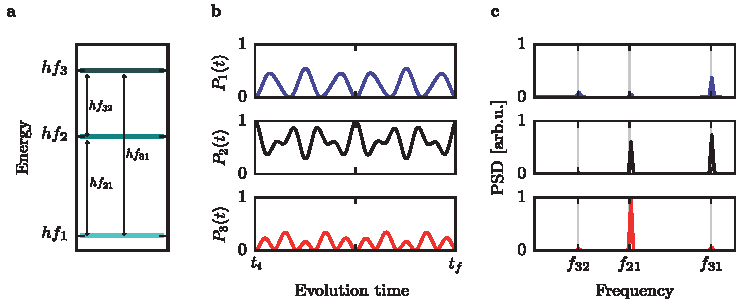
\includegraphics{Figures/Chapter5/Fig1.pdf}
		\caption[Operating principle of Fourier spectroscopy]
		{
			{\bf a.} Eigenenergies of a three-level system described by $\hat{H}'(\Omega_1,\Omega_2,\Omega_3)$. 
			{\bf b.} The system is prepared in $\ket{\psi_2}$ and subjected to $\hat{H}'$ at time $t_i$. The three panels show the occupation probabilities of the states $\ket{\psi_1}$ (blue), $\ket{\psi_2}$ (black), and $\ket{\psi_3}$ (red) in the measurement basis, for evolution times up to $t_f$. 
			{\bf c.} Power spectral density of the occupation probabilities from panel b. The three peaks in the Fourier spectra correspond to the energy differences present in panel a.
		\label{fig:Figure1}}
	\end{center}
\end{figure*}
%
We focus on a system where we can measure the occupation probabilities of a set of orthonormal states $\{\ket{\psi_i}\}$ that fully span the accessible Hilbert space of the system. We then consider the time evolution of an arbitrary initial state $\ket{\Psi_0}=\sum\limits_{i}a_i\ket{\psi_i}$ as governed by a Hamiltonian $\hat{H}'(\{\Omega_i \})$ and observe the occupation probabilities of the $\{\ket{\psi_i}\}$ states of the measurement basis as a function of time. When $\hat{H}'$ is applied, the evolution of the initial state is $\ket{\Psi(t)}=\sum\limits_{i,j}a_ic_{i,j}e^{-iE'_jt/\hbar}\ket{\psi'_j}$, where $E'_j$ and $\ket{\psi'_j}$ are the eigenenergies and eigenstates of $\hat{H}'$, and $c_{i,j}(t)=\braket{\psi_i}{\psi'_j}$. The probability 
%
\begin{align}
P_k(t)=&|\braket{\psi_k}{\Psi(t)}|^2=\lvert\sum\limits_{i,j}a_ic_{i,j}c^{*}_{j,k}e^{-iE'_jt/\hbar}\rvert^2
\label{Eq:Probability}
\end{align}
%
of finding the system in a state $\ket{\psi_k}$ of the measurement basis can be expressed as a sum of oscillatory components, with amplitude given by the magnitude of the overlap integrals between the initial state and the eigenvalues of $\hat{H}'$
\begin{align}
%P_k(t)=\tilde{a}_k+\sum\limits_{i\neq j}\tilde{b}_{i,j,k}\cos(2\pi f_{j,j'}t),
P_k(t)=1+\sum\limits_{i,j\neq l} 2\lvert a_i^2c_{i,j}c_{j,k}c_{i,l}c_{l,k}\rvert \cos(2\pi f_{j,l}t),
\end{align}
where $f_{j,l}=(E'_{j}-E'_{l})/h$ is the frequency associated with the energy difference of two eigenstates of the Hamiltonian.
Fourier spectroscopy relies on measuring the populations on each state of the measurement basis as a function of time and extracting the different frequency components $f_{j,l}$ directly by computing the discrete Fourier transform. The bandwidth and frequency resolution of the measurement are determined by the total sampling time and the number of samples. For $N$ samples separated by a time interval $\Delta t$, the highest resolved frequency will be $f_{\mathrm{bw}}=1/2\Delta t$, with resolution $\Delta f=1/\Delta tN$. This resolution can be decreased if the Fourier transform is calculated using certain types of windowing functions that enhance signal to noise ratio.  Any  higher frequency  $f>f_{\mathrm{bw}}$ will be aliased and measured in the Fourier spectrum as $f_{\mathrm{alias}}=\vert f - m/\Delta t \vert$, where $m$ is an integer. If interactions are present in the system, the dynamics get modified in a time scale given by the magnitude of the interactions, giving an additional constraint to the smallest frequency components of a single particle Hamiltonian that can be resolved with our technique.

Figure~\ref{fig:Figure1} illustrates the principle of Fourier spectroscopy for a three level system, initially prepared in the state $\ket{\Psi_0}=\ket{\psi_2}$, subject to the Hamiltonian
%
\begin{equation}
\hat{H}'=\begin{pmatrix}
E_1 & 0 & 0  \\
0 & E_2 & 0  \\
0 & 0 & E_3 \\
\end{pmatrix}
+\hbar\begin{pmatrix}
0 & \Omega_1 & \Omega_2  \\
\Omega_1^{*} & 0 & \Omega_3  \\
\Omega_2^{*} & \Omega_3^{*} & 0
\end{pmatrix},
\end{equation}
%
where we measure the occupation probability as a function of time for each of the $\{\ket{\psi_1}, \ket{\psi_2},\ket{\psi_3}\}$ states. The three eigenenergies $E'_i=hf_i$ that result from diagonalizing $\hat{H}'$are displayed in Figure~\ref{fig:Figure1}a. The three energy differences $hf_{jj'}$ between the levels determine the oscillation frequencies of the occupation probabilities, as can be seen in Figure~\ref{fig:Figure1}b. Finally, Figure~\ref{fig:Figure1}c shows a plot of the power spectral densities (PSD) with three peaks corresponding to the three relative energies of $\hat{H}'$. 
%
\section{Measuring the SOC dispersion with Fourier transform spectroscopy}
\label{sec:fs-exp}

We applied the Fourier transform spectroscopy technique to measure the dispersion relation of spin-1 BECs with an equal superposition of Rashba and Dresselhaus SOC, and tunable SOC strength.

\subsection{System}

\sloppy All of our experiments started with BECs containing about $4\times 10^4$ atoms in the $\ket{f=1,m_F=-1}$ hyperfine state. The experiments described in Section~\ref{sec:application_of_fs} were performed in an optical dipole trap with frequencies $(\omega_x,\omega_y,\omega_z)/2\pi=(42(3),34(2),133(3))\Hz$. We later modified the trapping frequencies in the $xy$ plane to try to make them more symmetric for the experiments described in Section~\ref{sec:effective_mass}. We broke the degeneracy of the three $m_F$ magnetic sub-levels by applying a $1.9893(3)\,$mT bias field along $\mathbf{e}_z$ that produced a $\omega_Z / 2\pi  = 14.000(2) \MHz$ Zeeman splitting, and a quadratic Zeeman shift $\epsilon$ that shifted the energy of $\ket{f=1,m_F=0}$ by $-h\times (28.45\, \kHz)$. We transfered atoms into the $\ket{f=1,m_F=0}$ state using ARP (see Section~\ref{sec:arp}) and then we monitored and stabilized the magnetic field using partial transfer absorption imaging  (Section~\ref{sec:ptai}) by applying a pair of $\unit[250]{\mu s}$ microwave pulses, each of them detuned by $\pm \unit[2]{kHz}$ from the $\ket{f=1, m_F=0}\leftrightarrow\ket{f=2, mf=1}$ transition.

\begin{figure*}[!ht]
	\begin{center}
		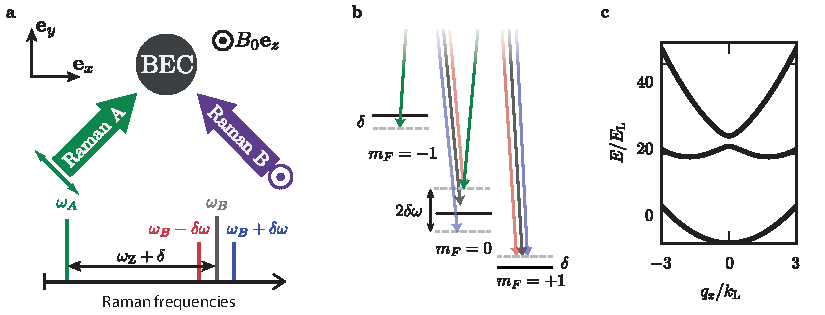
\includegraphics{Figures/Chapter5/Fig2.pdf}
		\caption[Experimental setup for engineering a tunable system with equal contributions of Rashba and Dresselhaus-type spin-orbit coupling]
		{
			{\bf a.} Setup. A bias magnetic field $B_0\ez$, with $B_0=1.9893$\,mT splits the hyperfine energy levels of the $f=1$ manifold of $^{87}$Rb by $\omega_Z/2\pi=14$\,MHz. A pair of cross polarized Raman beams propagating along $\ex+\ey$ and $\ex-\ey$ couple the atoms' momentum and spin states. 
			{\bf b.} The Raman frequencies are set to $\omega_A=\omega_L+\delta$ and $\omega_B=\omega_L+\omega_Z$. We add frequency sidebands to $\omega_B$, separated by $\pm \delta\omega$. The amplitude modulation from the interference between the multiple frequency components results in tunable SOC.
			{\bf c.} SOC dispersion for Raman coupling strength $\Omega_0=12E_{\mathrm{L}}$ and $\Omega=0$, on four photon resonance.
		\label{fig:Figure2}}
	\end{center}
\end{figure*}

We induced spin-orbit coupling using a pair of intersecting, cross polarized Raman laser beams propagating along $\mathbf{e}_x+\mathbf{e}_y$ and $\mathbf{e}_x-\mathbf{e}_y$, as shown in Figure~\ref{fig:Figure2}a and b. The beams had angular frequency $\omega_A=\omega_L+\delta$ and $\omega_B=\omega_L+\omega_Z$, where $2\delta$ is the, experimentally controllable, detuning from four photon resonance between $m_F=-1$ and $m_F=+1$. 

Our system was well described by the Hamiltonian including atom-light interaction along with the kinetic contribution
 
 \begin{align}
 \begin{split}
 \hat{H}_{\mathrm{SOC}} = &\frac{\hbar^2q_x^2}{2m} + \alpha q_x\hat{F}_z  + 4E_{\mathrm{L}}\hat{\mathbb{1}} + \hbar\Omega_{\mathrm{R}}\hat{F}_x  +(4E_{\mathrm{L}}-\epsilon)(\hat{F}_z^2-\hat{\mathbb{1}}) +\hbar\delta\hat{F}_z,
 \label{Eq:SOCone}
 \end{split}
 \end{align}
 %
where $q$ is the quasimomentum, $\hat{F}_{x,y,z}$ are the spin-1 angular momentum matrices,  $\alpha=\hbar^2k_{\mathrm{L}}/m$ is the SOC strength, and $\Omega_{\mathrm{R}}$ is the Raman coupling strength, proportional to the Raman laser intensity. The Raman field coupled $\ket{m_F=0,\, q=q_x}$ to $\ket{m_F=\pm1,\, q=q_x\mp 2k_{\mathrm{L}}}$, generating a spin change of $\Delta m_F=\pm1$ and imparting a $\mp 2k_{\mathrm{L}}$ momentum. The eigenstates of $\hat{H}_{\mathrm{SOC}}$ were linear combinations of these states and $\ket{m_F=0,\,q=q_x}$, and the set $\{\ket{m_F,q}\}$ constituted the measurement basis for Fourier transform spectroscopy.

Figure \ref{fig:Figure2}c shows a typical band structure of our spin-1 SOC system as a function of quasimomentum for a large and negative quadratic Zeeman shift $-\epsilon>4E_{\mathrm{L}}$. In this parameter regime, the ground state band had a nearly harmonic dispersion with an effective mass $m^{*} = \hbar^2[d^2E(k_x)/d^2x]^{-1}$, only slightly different from that of a free atom. 

\subsection{Tunable SOC}
We engineered a highly tunable dispersion relation in which we could independently control the size of the gap at $q_x=0$ as well as the SOC strength $\alpha$ by adding frequency sidebands to one of the Raman beams. The state of the system could change from $\ket{m_F=-1,\,q=q_x+2k_{\rm{L}}}$ to  $\ket{m_F=1,\,q=q_x-2k_{\mathrm{L}}}$ by absorbing a red detuned photon first followed by a blue detuned photon and vice versa, in a similar way to the M\o lmer-S\o rensen entangling gate in trapped ion systems \cite{sorensen_entanglement_2000}. When we set the angular frequencies of the sidebands to $\omega=\omega_{\mathrm{A}}+\omega_Z \pm \delta\omega$, the Hamiltonian (Equation~\ref{Eq:SOCone}) acquired a time-dependent coupling $\Omega_{\mathrm{R}}(t)=\Omega_0 + \Omega\cos(\delta\omega t)$. This periodically driven system was well described by Floquet theory \cite{floquet_sur_1883} (see Section~\ref{sec:Floquet_theory}). Figure~\ref{fig:Floquet} shows the spectrum of Floquet quasi-energies for a system described by Equation~\ref{Eq:SOCone} where $\Omega_{\rm R}$ oscillated with angular frequency $\delta\omega$. 
%
\begin{figure*}[htb]
	\begin{center}
		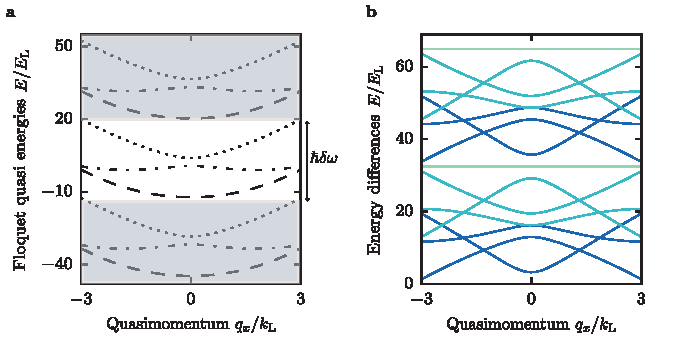
\includegraphics{Figures/Chapter5/Fig3.pdf}
		\caption[Floquet quasi-energy spectrum of a three-level system with spin-orbit coupling and periodic coupling strength]
		{
			{\bf a.} Floquet quasi-energies of a three level Hamiltonian with SOC and time periodic coupling strength. The quasi-energies are grouped into manifolds consisting of three levels that get repeated with a periodicity equal to $\hbar\delta\omega$.
%
			{\bf b.} Energy differences of the Floquet quasi-energies. Each color represents the energy difference, separated by a fixed number of neighboring levels. When the number of neighboring levels is a multiple of 3, the energy differences are straight lines, a result of the periodic structure of the Floquet manifolds. 
		\label{fig:Floquet}}
	\end{center}
\end{figure*}

We found an effective time-independent Hamiltonian using a unitary transformation $\hat{U}(t)$ and applying a RWA. The time evolution of the transformed wave function  $\ket{\psi'}=\hat{U}^{\dag}\ket{\psi}$ was given by the time dependent Schr\"odinger equation for the Hamiltonian $\hat{H}'=\hat{U}^{\dag}\hat{H}\hat{U}-i\hbar\hat{U}^{\dag}\partial_t\hat{U}$. We used 
\begin{equation}
\hat{U}(t)=\mathrm{exp}[-i\frac{\Omega}{\delta\omega}\sin(\delta\omega t)\hat{F}_x]
\end{equation}
%
\sloppy so that $i\hbar\hat{U}^{\dag}\partial_t\hat{U}=\hbar\Omega_{\rm R}(t)\fx$. The transformed Hamiltonian $\hat{H}'(t)$ had terms proportional to $\sin(\Omega/\delta\omega\sin(\delta\omega t))$, $\sin^2(\Omega/\delta\omega\sin(\delta\omega t))$, $\cos(\Omega/\delta\omega\sin(\delta\omega t))$ and $\cos^2(\Omega/\delta\omega\sin(\delta\omega t))$ which we simplified using the Jacobi-Anger expansion
\begin{align*}
&\cos(z\sin\theta)= J_0(z) + 2\sum_{n=1}^{\infty}J_{2n}(z)\cos(2n\theta) \approx J_0(z) \\
&\sin(z\sin\theta)= 2\sum_{n=0}^{\infty}J_{2n+1}(z)\sin((2n+1)\theta) \approx 0,
\end{align*} 
%
 where $J_n$ is the the $n$th order Bessel function of the first kind and we neglected the `fast' terms proportional to $\cos(2n\theta)$ and $\sin((2n+1)\theta)$, essentially performing a RWA.

This approximation is valid for $\hbar\delta\omega > \vert\epsilon\vert+12E_{\rm{L}}$ and $\vert q_x\vert \leq 2\kl$ so that quasi-energy manifolds are well separated as in Figure~\ref{fig:Floquet}a. The resulting Hamiltonian retained the form of Equation~\ref{Eq:SOCone} with renormalized coefficients and an additional coupling term
%
\begin{align}
\begin{split}
\hat{H}_{Fl} = &\hat{H}_{SOC}(q,\Omega_0,\tilde{\alpha},\tilde{\delta},\tilde{\epsilon}) + \tilde{\Omega}\hat{F}_{xz},
\label{Eq:SOCeff}
\end{split}
\end{align}
%
where $\tilde{\alpha}= J_0(\Omega/\delta\omega)\alpha$, $\tilde{\Omega}=1/4(\epsilon+4E_{\mathrm{L}}) [J_0(2\Omega/\delta\omega)-1]$, $\tilde{\delta}=J_0(\Omega/\delta\omega)\delta$, and $\tilde{\epsilon}= 1/4(4E_{\mathrm{L}}-\epsilon) -
1/4(4E_{\mathrm{L}} + 3 \epsilon) J_0( 2\Omega/\delta\omega)$. $\hat{F}_{xz}$ is the $\hat{\lambda}_4$ Gell-Mann matrix that directly couples $\ket{m_F=-1, q=q_x+2k_{\mathrm{L}}}$ and $\ket{m_F=+1, q=q_x-2k_{\mathrm{L}}}$ states. The experimentally tunable parameters $\delta\omega$, $\Omega$ and $\Omega_0$ can be used to tune the SOC dispersion.

\subsection{Application of Fourier spectroscopy}
\label{sec:application_of_fs}

We used Fourier transform spectroscopy to measure the spectrum of the SOC Hamiltonian (Equation~\ref{Eq:SOCeff}) for three coupling regimes: (i) $\Omega_0\neq0$ and $\Omega=0$, (ii)  $\Omega_0=0$ and $\Omega\neq0$ and (iii) $\Omega_0\neq0$ and $\Omega\neq0$. We turned on the Raman laser non-adiabatically, in approximately $1	\,\mu\mathrm{s}$. We let the system evolve subject to $\hat{H}_{\mathrm{SOC}}$ for up to $900\, \mathrm{\mu s}$, and then turned off the laser while releasing the atoms from the optical dipole trap. We resolved the spin and momentum distribution using a Stern-Gerlach gradient and a $\unit[21]{\ms}$ TOF which allowed us to measure the fraction of atoms in each state of the measurement basis $\{\ket{m_F, q}\}$. We chose the density of sampling points and the maximum evolution time so that the bandwidth of the Fourier transform was comparable to, or larger than, the highest frequency in the evolution of the system while maximizing resolution. Experimental decoherence resulting in loss of contrast of the oscillations due to magnetic field noise and small magnetic field gradients present in our apparatus, was an additional constraint that became significant around 1 ms. 

Working with a BEC with $k=0$ gave us access to only a single point in the dispersion relation. In order to map the full spin and momentum dependent dispersion relation of $\hat{H}_{\mathrm{SOC}}$, we measured the time dependent occupation probabilities at a fixed Raman coupling strength and different values of Raman detuning $\delta$ for the same initial state. The detuning corresponded to the Doppler shift experienced by atoms moving relative to a light source with quasimomentum $q_x/k_{\mathrm{L}}=\hbar\delta/4E_{\mathrm{L}}$. We controlled the frequency and the detuning of the Raman beams using two AOMs, one of which was driven by up to three phase coherent frequencies (the carrier frequency plus two sidebands). For each of the three coupling cases that we measured, we applied the Raman beams at detuning values within the interval $\pm 12 E_{\mathrm{L}}$ which corresponds to quasimomentum values $\pm 3k_{\mathrm{L}}$.

This approach of changing detuning rather than using atoms with non-zero quasimomentum had the advantage that the state preparation was very reliable (making BECs at rest is easy\footnote{Well, nothing in the lab is really `easy'...}!) and we got very good signal to noise ratios due to the relatively high densities of the BECs. The downside was that if one is interested in looking at a large range of different momenta it can take a long time to repeat each experiment for different detuning values. In subsequent implementations of Fourier transform spectroscopy (Chapter~\ref{ch:Rashba} and~\cite{anderson_realization_2019}) we sacrificed some signal to noise ratio for speed and used the momentum distribution of non-condensed atoms to parallelize our measurements. 

% For $\hat{H}_{\mathrm{SOC}}$, momentum and detuning are equivalent up to a numerical factor, $\delta/E_{\mathrm{L}}=4q_x/k_{\mathrm{L}}$, since the detuning term $\delta\hat{F}_z$ and the momentum term $\alpha\hat{q}_x\hat{F}_z$ have the same effect in the relative energies. This relation follows from the Doppler shift of the light frequency experienced by atoms moving relative to a light source: a stationary BEC in the laboratory reference frame dressed by a detuned laser field is equivalent to a moving BEC and a resonant laser field.

\begin{figure*}[!htb]
	\begin{center}
		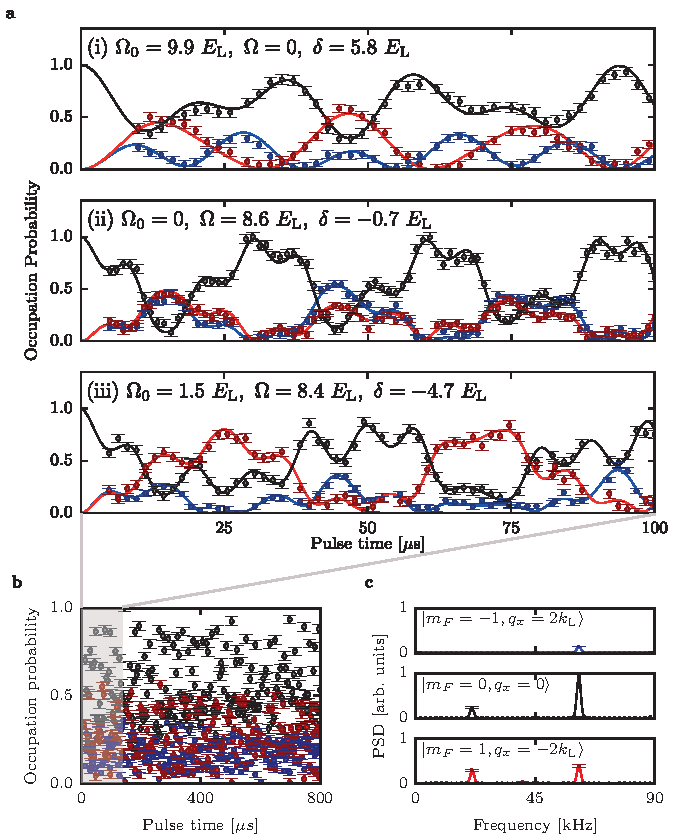
\includegraphics{Figures/Chapter5/Fig5.pdf}
		\caption[Time evolution and Fourier transforms of a SOC system]
		{{\bf a.}
		Occupation probability for the three states in the measurement basis $\ket{m_F=-1, q=q_x+2\kl}$ (blue), $\ket{m_F=0,q=q_x}$ (black), and $\ket{m_F=+1,q=q_x-2\kl}$(red),  following unitary evolution under $\hat{H}_{\mathrm{SOC}}$ for times up to 100 $\mu s$ at different spin-orbit coupling regimes: (i) $\Omega_0=9.9 E_{\mathrm{L}}$, $\Omega=04$,  $\delta=5.8 E_{\mathrm{L}}$, (ii) $\Omega_0=0$, $\Omega=8.6\,E_{\mathrm{L}}$,  $\delta=-0.7\,E_{\mathrm{L}}$, $\delta\omega=\epsilon+12\,E_{\mathrm{L}}$, and (iii) $\Omega_0=1.5\,E_{\mathrm{L}}$, $\Omega=8.4\, E_{\mathrm{L}}$,  $\delta=-4.7\,E_{\mathrm{L}}$, $\delta\omega=\epsilon+17\,E_{\mathrm{L}}$.
		{\bf b.} Occupation probability for long pulsing up to 800 $\mu$s for parameters as in (iii). 
		{\bf c.} Power spectral density of the occupation probability. We subtract the mean value of each probability before taking the Fourier transform to remove peaks at $f=0$. The peaks in the PSD then correspond to the relative eigenenergies of $\hat{H}_{SOC}$.
		}
		\label{fig:Figure5}
	\end{center}
\end{figure*}
%
We mapped the band structure of SOC atoms for three different coupling regimes. Figure~\ref{fig:Figure5}a shows representative traces of the measured occupation probabilities for short evolution times along with fits to the unitary evolution given by $\hat{H}_{\mathrm{SOC}}$ with $\delta$, $\Omega_0$, and $\Omega$ as free parameters. The fit parameters agree well with independent microwave and Raman power calibrations. In the lower two panels, where the Raman coupling strength was periodically modulated, the occupation probabilities oscillated with more than three frequencies since the full description of the system was given by a Floquet quasi-energy spectrum. Figure~\ref{fig:Figure5}b,c shows the occupation probabilities for the parameter regime (iii) for longer evolution times along with the PSD of the occupation probability of each spin state. 



\begin{figure}[!ht]
	\begin{center}
		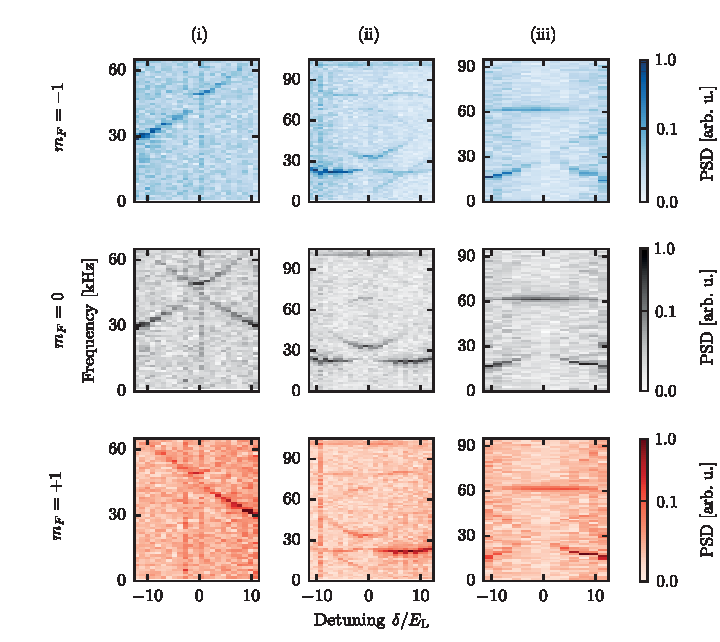
\includegraphics[width=4.8in]{Figures/Chapter5/Fig6a.pdf}
		\caption[Power spectral density of the time dependent occupation probability for each state in the measurement basis for three coupling regimes]
		{
			 Power spectral density of the time dependent occupation probability for each state in the measurement basis for three coupling regimes:
			{ (Left)} $\Omega_0=9.9 E_{\mathrm{L}}$, $\Omega=0$,
			{ (Center)} $\Omega_0=0$, $\Omega=8.6 E_{\mathrm{L}}$,  $\delta\omega=\epsilon+12 E_{\mathrm{L}}$, and
			{ (Right)} $\Omega_0=4.9 E_{\mathrm{L}}$, $\Omega=8.4 E_{\mathrm{L}}$,  $\delta\omega=\epsilon+17 E_{\mathrm{L}}$. Each panel is normalized to peak amplitude to highlight small amplitude features in the PSD of the periodically driven SOC, and the highest value on the frequency axis corresponds to the FFT bandwidth.
		}
		\label{fig:Figure6a}
	\end{center}
\end{figure}

We used a non-uniform fast Fourier transform algorithm (NUFFT) on a square window to obtain the power spectral density of the occupation probabilities since our data points were not always evenly spaced because of imperfect imaging shots. The heights of the peaks in the PSD are related to the magnitude of the overlap integrals between the initial state and the Raman dressed states. Figure~\ref{fig:Figure5}c shows the raw PSD of the time evolution of the system under $\hat{H}_{\mathrm{SOC}}$ for a given Raman coupling strength and detuning. We put together all the PSDs for the three coupling regimes in the spectra shown in Figure~\ref{fig:Figure6a}. Each column corresponds to a different coupling regime and the colors represent the different spin states of the measurement basis. The spectra show that some overlap integrals vanish near $\delta=0$, which is manifested as missing peaks in the PSD. The periodic structure of the Floquet quasi-energy spectrum gave rise to peaks at constant frequencies of $\delta\omega$ and $2\delta\omega$ independently of the Raman detuning, and a structure that is symmetric about the frequencies $2\pi f_1=\delta\omega/2$ and $2\pi f_2=\delta\omega$. A reader is interested in seeing another nice experiment where the Floquet quasienergy spectrum becomes can be visualized is advised to see~\cite{deng_observation_2015}.


\subsection{Effective mass}
\label{sec:effective_mass}

Fourier transform spectroscopy only gives access to the relative energies of a Hamiltonian. If we want to recover the absolute energies we need to have an additional energy reference. The particular Hamiltonian $\hat{H}_{SOC}$ had a ground state with a nearly quadratic dispersion. We measured its effective mass to obtain the ground state energy which we used as a reference to recover the absolute energies. 

We measured the effective mass of the Raman dressed atoms by adiabatically preparing the BEC in the lowest eigenstate and inducing dipole oscillations~\cite{Pethick}. The effective mass of the dressed atoms was related to the bare mass $m$ and the bare and dressed trapping frequencies $\omega$ and $\omega^{*}$ along the Raman recoil direction by the ratio $m^{*}/m=(\omega/\omega^{*})^2$. We measured this ratio following~\cite{lin_synthetic_2011}. To induce the oscillations we started in  $\ket{m_F=0,\, k_x=0}$ state and adiabatically turned on the Raman laser in $10\,\mathrm{ms}$ while simultaneously ramping the detuning to $\delta\approx0.5\,\El$ which shifted the minima in the ground state energy away from zero quasi-momentum. We suddenly brought the field back to resonance causing an abrupt change in the dispersion relation that excited the dipole mode of the BEC. To obtain the bare state $\omega$ we only used the Raman beams to induce the oscillations and then subsequently turned off the beams while the BEC oscillated in the dipole trap and to obtain $\omega^*$ the Raman beams were kept on the whole time.
For this set of measurements, we adjusted our optical dipole trap to give new trapping frequencies $(\omega_x, \omega_y, \omega_z)/2\pi=(35.6(4), 32.2(3), 133(3))\,\Hz$, nominally symmetric in the plane defined by $\ex$ and $\ey$. 

The Raman beams were co-propagating with the optical dipole trap beams; therefore, the primary axes of the dipole trap frequencies were at a $45^{\circ}$ angle with respect to the direction of $\mathbf{k}_{\mathrm{L}}$. The kinetic and potential terms in the Hamiltonian including the contribution of the Raman and optical dipole trap were

\begin{align}
\hat{H}_{\perp}= &\frac{\hbar^2q_x^2}{2m^{*}} + \frac{\hbar^2q_y^2}{2m}+\frac{m}{2}[\omega_{x'}^2x'^2+\omega_y'^2y'^2] \nonumber \\
= & \frac{\hbar^2}{2m^{\star}}k_x^2 + \frac{1}{2m}k_y^2+\frac{m}{4}[(\omega_{x'}^2+\omega_{y'}^2)(x^2+y^2)+2xy(\omega_{x'}^2-\omega_{y'}^2)],
\end{align}
%
where $x'=(x+y)/\sqrt{2}$ and  $y'=(x-y)/\sqrt{2}$ are position coordinates rotated by $45^{\circ}$ . For an axially symmetric trap with $\omega_{x'}=\omega_{y'}$, the frequency of oscillation along the Raman recoil direction  is 

\begin{equation}
\omega_x^2=\frac{m}{2m^{*}}(\omega_{x'}^2+\omega_{y'}^2).
\label{Eq:meff}
\end{equation}

Our trap had a small $3.4$\,Hz asymmetry and there was some coupling of the motion along the axis perpendicular to $\k_{\rm L}$ which becomes more significant at larger values of the effective mass. The sampling times for the measurements were small compared to the trap asymmetry and we can locally approximate the motion of the atoms by a simple harmonic function with a frequency along $\ex$ given by Equation~\ref{Eq:meff}.

Figure~\ref{fig:Figure4} shows the dipole oscillations along the $\mathbf{e}_{x}$ and $\mathbf{e}_{y}$ directions for the three different coupling regimes we explored, as well as the bare state motion. The resulting mass ratios for the three coupling regimes are $m/m^{*}=$  (i) $1.04(8)$, (ii) $0.71(7)$, and (iii) $0.62(4)$.
\begin{figure*}[!ht]
	\begin{center}
		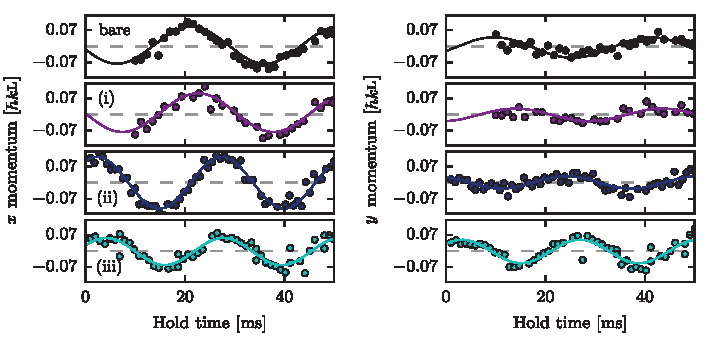
\includegraphics{Figures/Chapter5/Fig4.pdf}
		\caption[Dipole oscillations of a spin-orbit coupled BEC in a dipole trap]
		{  Oscillation of the BEC in the dipole trap along the  recoil directions $\mathbf{e}_{x}$ and  $\mathbf{e}_{y}$ for (top) bare atoms, and the three parameter regimes that we explored (i), (ii), and (iii).  We believe that the observed low amplitude oscillations along $\ey$ are due to the initial detuning ramp not being fully adiabatic. 
		\label{fig:Figure4}}
	\end{center}
\end{figure*}

\subsection{Measured dispersions}

Figure \ref{fig:Figure7} explains in detail the interpretation of the multiple peaks in the PSD and the steps that were taken to recover the dispersion relation using the effective mass and the Fourier spectra. The red line in Figure~\ref{fig:Figure7}a represents a level within a Floquet manifold that has the largest overlap integral with the initial $\ket{m_F=0, q=0}$ state. The peaks in the PSD correspond to energy differences between the marked level and the levels in neighboring Floquet manifolds pointed by the colored arrows. We show the theoretically computed energy differences on top of the measured PSD in panel b. The lowest frequency dominant peaks of the PSD correspond to energy differences with the adjacent lower Floquet manifold. To properly recover the SOC dispersion we shifted the PSD by a negative quadratic term $-\hbar^2q_x^2/2m^{*}$ as we show on panel c. We finally invert the frequency axis and shift it by $\delta\omega$. %Including the effective mass to reconstruct the spectrum of the time-independent SOC case, amounts to shifting the PSD by a positive quadratic term.
\begin{figure*}[!ht]
	\begin{center}
		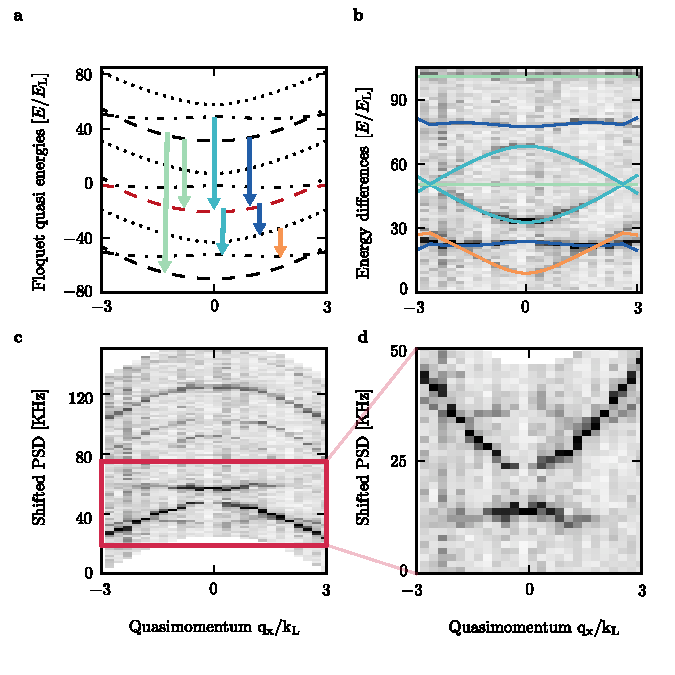
\includegraphics{Figures/Chapter5/Fig7.pdf}
		\caption[Converting energy differences into absolute energies]
		{  {\bf a} Floquet quasi-energy spectrum of a SOC Hamiltonian with periodic coupling strength. The red line represents the eigenstate that has the largest overlap with the initial $\ket{m_F=0}$ state. The arrows indicate the energies of the states that have non-zero overlap with the initial state and can be measured with Fourier transform spectroscopy.
		{\bf b} PSD of the occupation probability and numerically calculated energy differences between the levels indicated by the arrows on panel a.
		{\bf c} PSD shifted by a quadratic term $-\hbar^2 q^2_x/2m^*$. The red box indicates the region of interest where we can recover the SOC spectrum.
		{\bf d} We invert the frequency axis and shift it by $\delta\omega$.   
		}
		\label{fig:Figure7}
	\end{center}
\end{figure*}

We obtained the characteristic dispersion of a SOC system after adding a quadratic term to the PSD, proportional to the measured effective mass and rescaling the detuning into recoil momentum units. We combined the PSD of the time evolution of the three $\ket{m_F}$ states to look at the spin dependence of the spectra. Figure \ref{fig:Figure6b} shows the measured dispersion relations as well as the Floquet quasi-energies calculated for the Hamiltonian parameters obtained from our calibrations. The spectral lines that can be resolved with our technique depend on the overlap integrals of the initial state with the target Hamiltonian eigenstates. Additional energies can be measured by repeating the experiment with different initial states. The spectral lines we were able to resolve are in good agreement with the calculated energies of the Hamiltonian. 
\begin{figure}[!ht]
	\begin{center}
		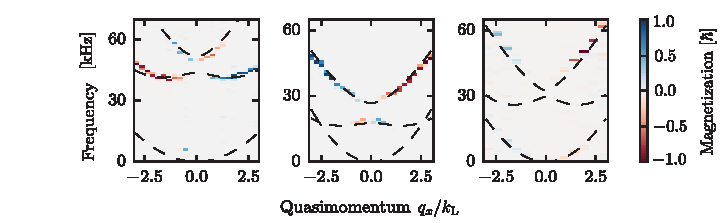
\includegraphics{Figures/Chapter5/Fig6b.pdf}
		\caption[Spin-dependent SOC dispersion for three different coupling regimes]
		{
			Spin-dependent SOC dispersion for three different coupling regimes. We combine the PSD of the occupation probability of the states $\ket{m_F=\pm 1, q_x=\mp 2k_{\mathrm{L}}}$, and shift each frequency by an amount proportional to the squared quasimomentum and the effective mass. The dashed lines are the calculated Floquet energies for the Hamiltonian using our calibration parameters. 
		}
		\label{fig:Figure6b}
	\end{center}
\end{figure}


\section*{Conclusion}

This chapter introduced the basic principles of the Fourier transform spectroscopy technique and used it to measure the spin and momentum dependent dispersion relation of a spin-1 spin-orbit coupled BEC. We additionally studied a periodically driven SOC system and found a rich Floquet quasi-energy spectrum. Our method can be applied generically to any system with long enough coherent evolution to resolve the energy scales of interest and could prove particularly useful to study systems where it is harder to predict or compute the exact energies, such as cold atom realizations of disordered or highly correlated systems \cite{eisert_quantum_2015}. In our lab, this technique has been used to study the spectrum of a Rashba spin-orbit coupled system~\cite{valdes-curiel_unconventional_2019} and of a fractional period adiabatic superlattice~\cite{anderson_realization_2019}.

Our main initial interest was to create tunable spin-orbit coupling and Fourier spectroscopy was conceived as a tool to characterize it. We realized that the use of Raman transitions from multiple frequency beams was equivalent to another experiment that achieved tunable SOC using amplitude modulated Raman coupling~\cite{jimenez-garcia_tunable_2015}.  %We therefore decided to focus on Fourier spectroscopy instead, a decision that turned out to be very fruitful for our lab as we continue to use this technique to characterize the spectrum of a variety of systems. 

% The idea of Fourier transform spectroscopy was born from a very different natured project. The project was originally conceived as a way to engineer tunable spin-orbit coupling using multiple-tone Raman transitions. The inspiration came from a previous project where we used multiple-tone Raman transitions to engineer a spin-1 spin-orbit coupled system whose ground state presented different magnetic phases~\cite{campbell_magnetic_2016}. Fourier spectroscopy was conceived as a new way to characterize the tunable dispersion relation resulting from our proposed coupling scheme. Unfortunately, we realized that this proposal was equivalent to another experiment that achieved tunable SOC using amplitude modulated Raman coupling~\cite{jimenez-garcia_tunable_2015}. We therefore decided to focus on studying Fourier spectroscopy instead, a decision that turned out to be very fruitful for our lab as we continue to use this technique to characterize the spectrum of a variety of systems. 








		% !TEX root = mainthesis.tex
%Chapter 6

\renewcommand{\thechapter}{6}

\chapter{Synthetic clock states}

\section{System}
\subsection{The xyz basis}
State decomposition, matrix elements, detuning dependence of energy something about resonantly coupling them

\section{Experiments}
\subsection{State preparation and deloading}
\subsection{Finding zero detuning}


\section{Robustness}

\section{Concatenated CCD}





		% !TEX root = mainthesis.tex
%Chapter 7

\renewcommand{\thechapter}{7}

\chapter{Topological order in quantum systems}
\label{ch:Topology}

Topological order can be found in a wide range of physical systems, from crystalline solids\cite{hasan_colloquium:_2010}, photonic meta-materials\cite{ozawa_topological_2019} and even atmospheric waves\cite{delplace_topological_2017} to optomechanic\cite{peano_topological_2015}, acoustic\cite{yang_topological_2015} and atomic systems\cite{cooper_topological_2019}. Topological systems are a robust foundation for creating quantized channels for transporting electrical current, light, and atmospheric disturbances. These topological effects can be quantified in terms of integer-valued invariants such as the Chern number, applicable to the quantum Hall effect\cite{thouless_quantized_1982,haldane_model_1988}, or the $\mathbb{Z}_2$ invariant suitable for topological insulators\cite{kane_$z_2$_2005}. 

The topology of Bloch bands defines integers that serve to both classify crystalline materials and precisely specify properties, such as conductivity, that are independent of small changes to lattice parameters\cite{hasan_colloquium:_2010}. Topologically non-trivial materials first found application in metrology with the definition of the von Klitzing constant as a standard of resistance, which is now applied in the realization of the kilogram\cite{newell_codata_2018}. Today, topological systems have found applications in the engineering of low loss optical waveguides\cite{ozawa_topological_2019} and present a promising path to quantum computation\cite{nayak_non-abelian_2008}. %\note{Not sure if I want to keep this paragraph as it is.}

We got interested in topology when working on a system with Rashba~\cite{bychkov_oscillatory_1984} type spin-orbit coupling in the lab. Our system had non-trivial topology but it broke from the usual mold of topological materials as it didn't have an underlying crystalline structure that conventionally yields to integer Chern numbers. 

Before describing our experiments to both engineer and characterize the unconventional topology of a Rashba spin-orbit coupled gas, in this Chapter I take a step back to describe the basic concepts of topology and its applications to the band theory of solids. The ideas of topology and how exactly one can connect donuts with band structures might feel a bit obscure and complicated for non-experts in the field. I wrote this Chapter with that in mind, with the hope that it can be followed by non-experts and provide some insight and intuition about this field. The concepts introduced in this Chapter will be necessary for understanding the results presented in Chapter~\ref{ch:Rashba}.
 
\section{Topology in mathematics} 

Topology is a branch of mathematics that studies continuity~\cite{differential_topology_and_geometry}. The most familiar example might be that of objects being continuously deformed into one another. For example, a donut can be continuously deformed into a coffee mug but if we want to deform it into a pretzel we need to poke more holes in it. This gives us some intuition that the donut and the mug must share the same topology, which is different from that of the pretzel. Topology also studies more abstract objects but I will limit the discussion to closed two-dimensional surfaces (manifolds) in three dimensions, which will be enough to provide some intuition when we define topological invariants for band structures in the following sections.  

The topology of 2D surfaces can be classified by the Euler characteristic, and it is related to the local Gaussian curvature of a surface by the Gauss-Bonet theorem. The Gaussian curvature can be interpreted in the following way: at any point $\x_0$ on a surface we can find a normal vector $\hat n$ that is orthogonal to the tangent plane of the surface (red arrow in Figure~\ref{fig:gauss_bonnet}). We can then define a family of planes containing $\hat n$ and the intersection between any of these planes and the surface defines a curve. If we perform a Taylor expansion of the curve around $\x_0$ the quadratic term defines what is known as the normal curvature $\kappa$. The orange and blue lines in Figure~\ref{fig:gauss_bonnet} are two examples of such curves and their curvatures correspond to the minimum and maximum value of the surface; they are what is known as the principal curvatures $\kappa_{min}$ and $\kappa_{max}$. The Gaussian curvature at any point of a surface is defined in terms of the principal curvatures as $K=\kappa_{min}\kappa_{max}$~\cite{differential_topology_and_geometry}.
%
\begin{figure*}[htb]
\begin{center}
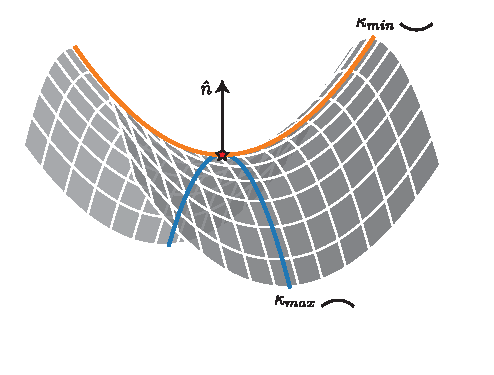
\includegraphics[]{Figures/Chapter7/gauss_bonnet.pdf}
\caption[The Gaussian curvature of a surface]{The intersection of planes containing the normal vector $\hat{n}$ at $\x_0$ (red star) and the gray surface define a family of curves. The minimum and maximum curvatures, corresponding to the orange and blue lines respectively, correspond to the principal curvatures of the surface at $\x_0$.}
\label{fig:gauss_bonnet}
\end{center}
\end{figure*}

The Gauss-Bonnet theorem states that the integral of the local Gaussian curvature over a closed surface is equal to the integer valued Euler characteristic
%
\begin{equation}
    \chi = \frac{1}{2\pi}\int_S K dA,
    \label{eq:euler_characteristic}
\end{equation}
%
which is related to the genus $g$ (number of holes or handles in the surface) by $\chi=2(1-g)$. The Gauss-Bonnet theorem is a very powerful result as it relates the local properties of a surface,the Gaussian curvature, with a global topological invariant, the Euler characteristic.

In the following sections I will introduce topological invariants in the context of condensed matter physics, which even though might seem a bit more abstract, their interpretation can be closely related to the concepts just defined in this section. 
\section{Topological order in condensed matter}

Just like topology classifies properties of geometric objects, one important task of condensed matter physics has been to classify phases of matter. Many of these phases, for example, magnetic or conducting phases, can be described in terms of order parameters related to spontaneously broken symmetries~\cite{landau_theory_1936}. However, in the past few decades, an increasing number of systems have been found where it is only possible to understand their phases and properties in terms of the underlying topology of their quantum states. This new paradigm of physics has been so important that in 2016 the Nobel prize in physics was awarded to David J. Thoules, F. Duncan M. Haldane and J. Michael Kosterlitz for the theoretical discoveries of topological phase transitions and topological phases of matter 

The effects of topology in condensed matter systems were first observed when von Klitzing and colleagues~\cite{klitzing_new_1980} measured the quantized Hall resistance in two-dimensional electron gases subjected to a strong perpendicular magnetic field. The effect can be understood semi-classically by thinking of the electrons' quantized cyclotron orbits\footnote{This is an intuitive but not very complete explanation of the quantum Hall effect, see \cite{tong_lectures_2016} if you want to learn more about this subject.} that give rise to Landau levels. If the Landau levels are filled then there is an energy gap separating two consecutive levels and the material acts as an insulator but if an electric field is applied the orbits drift and the electrons will be `skipping orbits' in the edge as can be seen in Figure~\ref{fig:quantum_hall}, giving rise to what is known as edge states.
% 
\begin{figure*}[htb]
\begin{center}
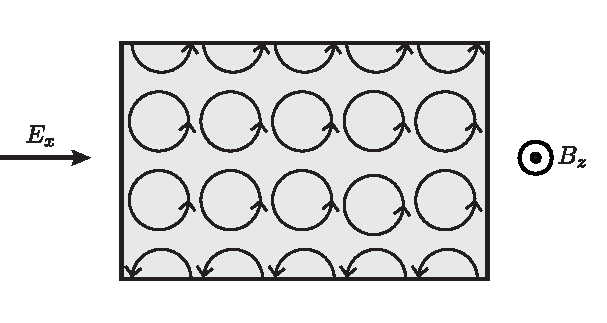
\includegraphics[]{Figures/Chapter7/quantum_hall.pdf}
\caption[The quantum Hall effect]{The quantum Hall effect. An electron gas is confined in a two-dimensional material and a strong magnetic field is applied perpendicular to the plane. The electrons on the bulk travel in cyclotron orbits while the electrons on the edge travel `skipping orbits'.}
\label{fig:quantum_hall}
\end{center}
\end{figure*}

In a seminal paper Thoules, Kohomoto, Nightingale, and den Nijs~\cite{thouless_quantized_1982} explained that the quantization of the Hall conductivity is determined by the underlying topology of the band structure. Just like the Euler characteristic defined in Equation~\ref{eq:euler_characteristic} classifies 2D solids that can be continuously deformed without opening or closing holes, there is a topological invariant that classifies band structures that can be deformed into one another without opening or closing an energy gap. This invariant, initially known as the `TKNN invariant', was later recognized by the mathematical physicist Bary Simon as the `first Chern class invariant from $U(1)$ fiber bundles'\footnote{See~\cite{geometry_topology_physics} if you want to dive into hardcore topology.}~\cite{simon_holonomy_1983} and the TKNN invariant became what is known today as the Chern number or Chern invariant. Another very valuable contribution from Simon's work was that he made the connection between the Chern number and the Berry's geometrical phase~\cite{berry_michael_victor_quantal_1984} which will be defined in the following sections and will allow us to make a physical interpretation of this otherwise abstract seeming topological invariant. 

\section{Berry phase and Berry curvature}
\label{sec:Berry phase and curvature}

A Berry or geometric phase is used to describe the phase acquired by a quantum state as it moves through a closed trajectory in parameter space. It plays a key role in topological band theory and can help provide a physical interpretation of the Chern number. 

Consider a Hamiltonian $\hat H$ that depends on a set of parameters $\r=(r_1, r_2, ...)$. If the parameters are slowly changed in time, the corresponding change in the system can be described by a path in parameter space $\r(t)$. The state $\ket{\psi(t)}$ evolves according to the time dependent Sch\"odinger equation and at any given time $t$ there is a basis that satisfies
%
\begin{equation}
    \hat H(\r)\ket{n(\r)}=E_n(\r)\ket{n(\r)}
    \label{eq:hamiltonian_eigenvectors}
\end{equation}
%
for $\r=\r(t)$. Suppose the system is initially in state $\ket{n(\r(t=0))}$, if the parameters are changed slowly such that the adiabatic theorem is valid, then at time $t$ the state of the system can be written as
%
\begin{equation}
    \ket{\psi(t)}=\exp\Big\{-\frac{i}{\hbar}\int_0^tdt'E_n(\r(t'))\Big\}\exp(i\gamma_n(t))\ket{n(\r(t))},
    \label{eq:berry_wf}
\end{equation}
%
where the first exponential term corresponds to a dynamical phase factor, and the second term is a geometric phase. By imposing that $\ket{\psi(t)}$ satisfies the time-dependent Schr\"odinger equation one finds that 
%
\begin{equation}
    \gamma_n(t)=i\braket{n(\r)}{\nabla_{\r}n(\r)}\cdot\dot{\r}(t),
\end{equation}
%
where the term
%
\begin{equation}
    \mathbf{A}_n(\r)=i\braket{n(\r)}{\nabla_{\r}n(\r)}
    \label{eq:berry_connection}
\end{equation}
%
 is usually referred to as the Berry connection\footnote{This is related to the connection defined in differential geometry that is used to describe things like parallel transport.} or the Berry vector potential for reasons that will become apparent. Because eigenvectors can only be defined up to a global phase, $\mathbf{A}$ is a gauge dependent quantity. If we make a gauge transformation such that $\ket{n(\k)}\rightarrow\e^{i\xi(\k)}\ket{n(\k)}$ then the Berry connection is also transformed as $\mathbf{A}_n(\k)\rightarrow\mathbf{A}_n(\k)-\nabla_{\k}\xi(\k)$. However if we integrate the Berry connection on a closed loop
%
\begin{equation}
    \gamma_n(\mathcal{C})=\oint_{\mathcal{C}} \mathbf{A}_n(\r)\cdot d\mathbf{l},
    \label{eq:berry_phase}
\end{equation}
%
we obtain the Berry phase which, unlike the Berry connection, is gauge independent (modulo $2\pi$). %It should also be noted that  $\gamma_n$ only depends on the geometry of the path and is independent of how it was traversed in time.

An alternative way to compute Berry's phase uses Stokes's theorem from vector calculus
%
\begin{align}
    \oint_{\mathcal{C}} \mathbf{A}_n\cdot d\mathbf{l}=&\int_{\mathcal{S}}\nabla\times\mathbf{A}_n\cdot d\mathbf{S} \nonumber \\
    =& \int_{\mathcal{S}}\mathbf{\Omega}_n\cdot d\mathbf{S},
    \label{eq:berry_connection}
\end{align}
%
where the vector field $\mathbf{\Omega}_n=\nabla\times\mathbf{A}_n$ is known as the Berry curvature or Berry field. By rewriting the Berry phase in this way, its resemblance with the definition of the Euler characteristic from Equation~\ref{eq:euler_characteristic} becomes apparent.

Using some vector calculus identities the Berry curvature can be rewritten as

\begin{align}
    \mathbf{\Omega}_n=&i[\nabla_{\r}\bra{n}]\times[\nabla_{\r}\ket{n}]\nonumber \\ 
    =& \sum_{j\neq n} i[\bra{n}\nabla_{\r}\ket{j}]\times[\bra{j}\nabla_{\r}\ket{n}] \nonumber \\
    =& i\sum_{j\neq n}\frac{\bra{n}\nabla_{\r}\hat{H}\ket{j}\times\bra{j}\nabla_{\r}\hat{H}\ket{n}}{(E_j-E_n)^2},
    \label{eq:alternative_berry_con}
\end{align}
%
where $\bra{n}\nabla_{\r}\ket{j}$ was replaced with $\bra{n}\nabla_{\r}\hat{H}\ket{j}/(E_j-E_n)$ by differentiating Equation~\ref{eq:hamiltonian_eigenvectors}. This expression shows that $\mathbf{\Omega}_n$ is a gauge independent quantity as it does not depend on the derivatives of a particular gauge choice for $\ket{n}$ but rather on $\nabla_{\r}\hat{H}$ which is gauge independent. Also we can see that $\mathbf{\Omega}_n$ becomes singular when there are degeneracies present in the Hamiltonian, and these degeneracies act as `sources' for the Berry curvature. Finally, even though the system may remain in state $\ket{n}$ during the adiabatic evolution, this expression for the Berry curvature makes it explicit that other eigenstates of the Hamiltonian have an influence in the Berry phase acquired. 

\subsection{Aharonov-Bohm phase as an example of a Berry's phase}

A familiar example of geometric phases is the Aharonov-Bohm phase~\cite{aharonov_significance_1959} gained by an electron moving along closed trajectories around a solenoid. This phase was initially conceived as a way of showing that in quantum mechanics magnetic vector potentials, typically conceived only as mathematical objects, can have a physical effect on the wave function. They considered a coherent electron beam split into two paths around a solenoid that produces a magnetic field $\mathbf{B}$ and later recombined as shown in Figure~\ref{fig:aharonov_bohm}. Outside the solenoid the magnetic field $\mathbf{B}=0$, but there can be a non-zero magnetic vector potential such that $\mathbf{B}=\nabla\times\mathbf{A}$. Even though the electron's trajectories are not modified by the presence of the solenoid, when looking at the interference pattern one finds that the two paths acquired different phases, and their difference is remarkably equal to magnetic flux piercing the area enclosed by the path of the electrons $\Delta\varphi = 2\pi \Phi_B/\Phi_0$, where $\Phi_0=h/e$ is the flux quantum. This Aharonov-Bohm phase can be interpreted as an example of a Berry phase in real space.

\begin{figure*}[htb]
\begin{center}
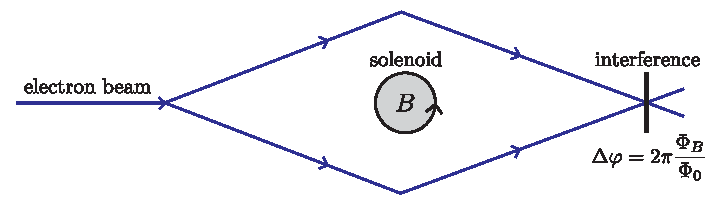
\includegraphics[]{Figures/Chapter7/aharonov_bohm.pdf}
\caption[The Aharonov-Bohm experiment]{The Aharonov-Bohm experiment. A coherent electron beam is split into two paths surrounding a solenoid which produces a non-zero magnetic field $\mathbf{B}$ inside the gray region and $\mathbf{B}=0$ outside. The two beams are later recombined and an interference pastern reveals a phase difference $\Delta\varphi = 2\pi \Phi_B/\Phi_0$ equal to the magnetic flux enclosed by the electron's path.}
\label{fig:aharonov_bohm}
\end{center}
\end{figure*}

For a charged particle in the presence of a vector potential, the momentum dependence of the free-particle Hamiltonian is modified $\mathbf{p}\rightarrow\mathbf{p}-q\mathbf{A}$ so that the wave function will depend on the magnetic vector potential as well. Using Equations~\ref{eq:berry_phase} and~\ref{eq:berry_connection} it can be shown that the Berry phase associated with a closed path around the solenoid is exactly equal to the Aharonov-Bohm phase: 
%
\begin{align}
    \gamma_n(\mathcal{C})=&\frac{e}{\hbar}\oint_{\mathcal{C}}\mathbf{A}(\mathbf{r})\cdot d\mathbf{r} \nonumber \\
    =& \frac{e}{\hbar}\int_{\mathcal{S}}\nabla\times\mathbf{A}\cdot d\mathbf{S} \nonumber \\
    =& \frac{e\Phi_B}{\hbar},
    \label{eq:aharonov_bohm_phase}
\end{align}

In this particular example, the Berry connection is exactly equal to the magnetic vector potential and the Berry curvature is the magnetic field. This gives us a very physical intuition for interpreting the Berry phase in terms of the `magnetic flux' from abstract sources of `magnetic fields' in parameter space.  

\subsection{Chern number}

The Chern number is conventionally used to describe the topology of materials which have an underlying crystalline structure. According to Bloch's theorem, the wave functions of a space periodic Hamiltonian can be written as $\ket{\psi(\k)}=e^{i\k\cdot\mathbf{r}}\ket{u(\k)}$\footnote{Very much like Floquet theory in momentum space}, where $\r$ is the position and $\k$ the crystal momentum. The wave functions $\ket{u(\k)}$ are periodic and therefore invariant under the displacement operator $\hat{D}(n\,d)\ket{u(\k)}=\ket{u(\k)}$ when $d$ is the unit cell size and $n$ an integer. If we define the Bloch Hamiltonian
%
\begin{equation}
    \hat{H}(\k)=e^{i\k\cdot\mathbf{r}}\hat{H} e^{-i\k\cdot\mathbf{r}}, 
\end{equation}
%
their eigenvectors are given by $\ket{u(\k)}$ and the eigenvalues define the band structure. Translational symmetry implies that $\hat{H}(\k+\mathbf{a})=\hat{H}(\k)$ where $\mathbf{a}$ is a reciprocal lattice vector. The crystal momentum or quasimomentum (in analogy to the Floquet quasienergy) is only defined within the periodic Brillouin zone and therefore can be mapped into a torus in $d$ dimensions if we glue the edges together.  

The Chern number of the $n$th band is defined as
%
\begin{equation}
    C_n=\frac{1}{2\pi}\int_{BZ}\mathbf{\Omega}_n\cdot  d\k,
    \label{eq:chern_number}
\end{equation}
%
where the relevant parameter space is crystal momentum and the surface of integration corresponds to the BZ (a torus). The definition of the Chern number is closely related to the Berry phase from Equation~\ref{eq:berry_connection}. For our previous example of a quantum Hall system, the integer proportionality factor in the quantized conductance is exactly equal to the Chern number. 

Just like two-dimensional surfaces are classified by the integral of their Gaussian curvature, the topology of Bloch bands and quantum systems, in general, is determined by the integral of the Berry curvature. Similarly, the integral connects local properties of a quantum system, the Berry connection, with a global topological invariant, the Chern number. One subtle difference is that the Euler characteristic is only determined by the surface (and its intrinsic Gaussian curvature) while the Chern number is defined both by a surface (the BZ) and an additional local curvature (the Berry curvature). By considering different lattice Hamiltonians one can obtain a different Berry curvature, but the geometry of the BZ and thereby the surface of integration is typically defined by a torus\footnote{In the next chapter we consider a case where this breaks down.}. This difference will be important later on when we describe the experiments performed to study a system with Rashba spin-orbit coupling where the unit cell size is taken to infinity (i.e. we remove the lattice).

\section{The bulk-edge correspondence principle}

Earlier I mentioned that topological systems provide very robust channels for transporting things like electrical current and light. Transport phenomena typically arise when there is a spatial interface between two topologically distinct phases. The electrons skipping orbits at the interface of a (topological) quantum Hall material and (trivial) vacuum are one example of this. Notice that for this particular example the modes propagate along a given direction, they are chiral. In general, one can expect to have modes moving along two directions, and the difference between the number of these modes $N_L - N_R$ is fixed and determined by the topology of the bulk states. The bulk-edge correspondence principle relates the difference in the number of these modes with the bulk topology of the materials at the interface:
%
\begin{equation}
    \Delta C=N_R - N_L
\end{equation}
%
where $\Delta C$ is the difference of Chern number on the interface. 

\section{Example: two-level model}
\label{sec:2_level_topology}

Many of the concepts introduced in the previous section can be readily applied and understood using a two-level model
%
\begin{equation}
    \hat{H}(\mathbf{k})= \mathbf{h}(\mathbf{k})\cdot\hat{\boldsymbol{\sigma}}
    \label{eq:2D_Hamiltonian}
\end{equation}
%
where $\hat{\boldsymbol{\sigma}}=(\sigma_x, \sigma_y, \sigma_z)$ are the Pauli matrices and $\mathbf{h}(\mathbf{k})=(h_x(\k),h_y(\k), h_z(\k))$ are functions of $\k$. This model has been used to describe a number of physical systems like graphene~\cite{haldane_model_1988} and spin-orbit coupled systems~\cite{bychkov_oscillatory_1984,dresselhaus_spin-orbit_1955}. Let us now consider the simple case $h(\k)=\k$, for which $\nabla_{\k}\hat{H}=\boldsymbol{\sigma}$ and using Equation~\ref{eq:alternative_berry_con} it can be shown that
%
\begin{equation}
    \mathbf{\Omega}=-\frac{\mathbf{h}}{2h^3}
    \label{eq:monopole}
\end{equation}
%
which can be recognized as the field of a Dirac monopole~\cite{dirac_paul_adrien_maurice_quantised_1931} with charge $-1/2$. The degeneracy in the energies that gives rise to the monopole is known as a Dirac point as the energies in that vicinity resemble the dispersion of a massless Dirac particle. In 2D materials where $\k$ is only defined within 2D plane $h_z$ corresponds to the mass of a Dirac particle but its effect on the Berry curvature is equivalent to that of moving the Dirac monopole along a fictitious $k_z$ dimension in a direction determined by the sign of $h_z$.

It follows from Equation~\ref{eq:monopole} that the Berry phase gained by moving along a closed path $\mathcal{C}$ is equal to the flux from the monopole in the surface enclosed by $\mathcal{C}$ as is shown in Figure~\ref{fig:solid_angle}. This connects nicely with our intuition from the Aharonov-Bohm effect. For a closed surface enclosing the Dirac point, the Chern number is an integer equal to 1. 
%
\begin{figure*}[htb]
\begin{center}
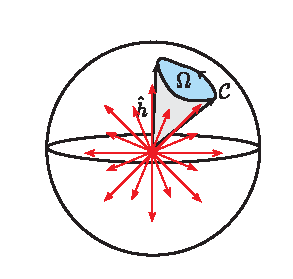
\includegraphics[]{Figures/Chapter7/solid_angle.pdf}
\caption[Graphical representation of Chern number]{For a two-level system, the Berry curvature from a Dirac point can be viewed as a Dirac monopole in momentum (parameter) space. The Chern number can be interpreted as the flux from the monopole on the solid angle subtended by the vector $\hat{h}(\k)$ or alternatively as the number of times $\hat{h}(\k)$ wraps around a unit sphere.}
\label{fig:solid_angle}
\end{center}
\end{figure*}

For a Hamiltonian with arbitrary $\mathbf{h}(\k)$ we can define a normalized vector $\hat{h}=\mathbf{h}/\vert\mathbf{h}\vert$ and the Chern number takes the form
%
\begin{equation}
    C=\frac{1}{4\pi}\int(\partial_{k_x}\hat{h}\times\partial_{k_y}\hat{h})\cdot\hat{h} \, d^2k
\end{equation}
%
which can be interpreted as the number of times that the vector $\hat{h}(\k)$ wraps around a unit sphere~\cite{kaufmann_notes_2016}, a quantity that is known as the winding number. Depending on the sign of $h_z$ the vector $\hat{h}(\k)$ will wrap around the north or south hemisphere, so to have integer valued Chern numbers, Dirac points must come in pairs. Luckily for lattice Hamiltonians this is guaranteed by the fermion doubling theorem~\cite{nielsen_adler-bell-jackiw_1983}. In Chapter~\ref{ch:Rashba} I describe an engineered system that has a single Dirac point. 

\section{Monopoles and Dirac strings}
\label{sec:Dirac_string}

We just gained some intuition about interpreting the Chern number as the flux from Dirac monopoles. But if we stick to our knowledge of electromagnetism we might remember that magnetic monopoles are forbidden since
%
\begin{equation}
    \nabla\cdot\mathbf{B}=\nabla\cdot(\nabla\times\mathbf{A})=0.
\end{equation}
%
So how is it possible to keep a vector potential and have $\nabla\cdot\mathbf{B}\neq0$? The solution to this problem was envisioned by Dirac~\cite{dirac_paul_adrien_maurice_quantised_1931} and is now called a Dirac string. If we consider a semi-infinitely long and infinitesimally thin solenoid, the magnetic field in the finite end will resemble that of a monopole as can be seen in Figure~\ref{fig:monopole}. This tiny solenoid corresponds to the Dirac string. 
%
\begin{figure*}[htb]
\begin{center}
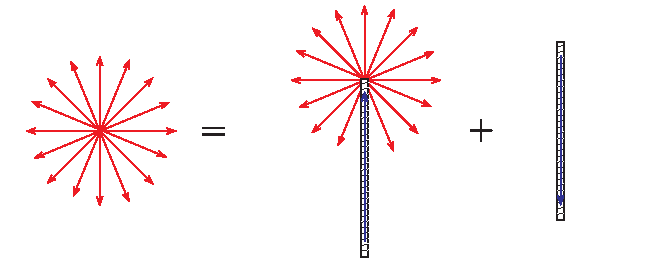
\includegraphics[]{Figures/Chapter7/monopole.pdf}
\caption[Graphical representation of Chern number]{For a two-level system, the Berry curvature from a Dirac point can be viewed as a Dirac monopole in momentum (parameter) space. The Chern number can be interpreted as the flux from the monopole on the solid angle subtended by the vector $\hat{h}(\k)$ or alternatively as the number of times $\hat{h}(\k)$ wraps around a unit sphere.}
\label{fig:monopole}
\end{center}
\end{figure*}
A more mathematical interpretation of these strings comes from the fact that in order to have $\nabla\cdot\mathbf{B}\neq 0$ the vector potential of a monopole must have `lines' where it becomes singular. For example, we can write for a particular gauge
%
\begin{equation}
    \mathbf{A}(\r)=g\frac{-y\ex+x\ey}{r(r+z)}
\end{equation}
%
which is singular at the Dirac string located at the negative $z$ axis where $z=-r$ . The orientation of the Dirac string is gauge dependent, something that should not surprise or bother us at this point. However, the physical effects of the Dirac string should be gauge independent, or in other words, the Aharonov-Bohm phase gained by a charged particle moving in a path that encloses the string should be an integer multiple of $2\pi$. This is argument gives rise to the Dirac charge quantization~\cite{dirac_paul_adrien_maurice_quantised_1931}, and in the context of topology, it guarantees that when we calculate the Berry phase by integrating the Berry connection (vector potential) along a path that encloses a Dirac string, its effect will be indistinguishable. 

\section{Conclusions}

Topology plays a very important role both in math and in physics. In this Chapter I reviewed the basic concepts of topology in the context of condensed matter physics that will be relevant for our experiments with unconventional topology. As a closing remark, Figure~\ref{fig:topology_analogies} summarizes the main concepts that were introduced and is a reminder that topological invariants are global properties defined in terms of integrals of local properties. Furthermore, we can use our intuition from electromagnetic theory to interpret topological invariants in quantum mechanics. 

 \begin{figure*}[htb]
\begin{center}
\includegraphics[]{Figures/Chapter7/topology_analogies.pdf}
\caption[Different topological invariants]{The Euler characteristic and the Chern number are topological invariants defined by integrals of local curvatures. The Aharonov-Bohm phase gives us physical intuition to interpret the Chern number as the flux from a `Berry field'.}
\label{fig:topology_analogies}
\end{center}
\end{figure*}

%%%%%%%%%%%%%%%%%%%%%%%%%%%%%%%%%%%%%%%%%%%%%%%%%%%%%%%%%%%%%%%
%
%Graveyard
%
%%%%%%%%%%%%%%%%%%%%%%%%%%%%%%%%%%%%%%%%%%%%%%%%%%%%%%%%%%%%%%%%

% In order for the field resulting from this string to be indistinguishable from that of a monopole, the Aharonov-Bohm phase gained by an electron moving around it has to be indistinguishable. For a monopole with charge $g$ this means that $2\pi N=\Phi_g/\Phi_0$

% A For this gauge choice, the $-z$ axis corresponds to the Dirac string. The orientation of the string might change for a different basis but if we demand that the field resulting from either of this vector potentials 


% I mentioned earlier that the Berry curvature from a Dirac point looks like a monopole and that the flux from this monopole on a closed surface is equal to the Chern number. This 
% If we try to write the vector potential for a monopole we will find that there is a line where it becomes singular. For example, for a monopole with charge g we can write
% %
% \begin{equation}
% 	\mathbf{A}(\r)=g\frac{-y\ex+x\ey}{r(r+z)}
% \end{equation}
% %
% which is singular at the south pole where $z=-r$. We could alternatively write 
% %
% \begin{equation}
% 	\mathbf{A}(\r)=g\frac{y\ex-x\ey}{r(r-z)}
% \end{equation}
% %
% which leads to the same 
% The existence of Dirac monopoles comes with some interesting consequences. A magnetic monopole can be thought of as the end of a semi-infinitely long and infinitesimally thin magnetic solenoid. In order for the field of the solenoid to be indistinguishable from that of a monopole, the Aharonov-Bohm phase gained by an electron moving around it has to be indistinguishable. For a monopole with charge $g$ this means that $2\pi N=\Phi_g/\Phi_0$

% . This thin solenoid can in fact be identified with  


% The existence of Dirac monopoles means that there has to be a singularity in the vector potential. 


% to be a Dirac string~\cite{dirac_paul_adrien_maurice_quantised_1931}. Dirac envisioned having an infinitesimally thin solenoid whose end looks like a magnetic charge. The monopole can only be identified as such if the thin solenoid is not experimentally detectable.

% Lets imagine for a moment 
% %
% \begin{equation}
% 	\int_{\mathcal{S}}\mathbf{B}\cdot d\mathbf{S}=q_m
% \end{equation}

% It is possible to find a magnetic vector potential 
% m This objects were conceived by Dirac as tiny solenoids
% If magnetic monopoles exist then electric charge must be quantized
% In electromagnetic theory 

% A consequence of the Berry connection being singular 

% This vector potential has one problem. It is singular at the north pole (z = r). In fact, one can prove that no matter which gauge one uses, there will always be a singularity point.

% Degeneracies as sources of Berry curvature field. There must therefore be Dirac strings as well..


% If there is inversion ($\mathcal{P}$) and time reversal ($\mathcal{T}$) symmetry $h_z(\k)=0$ and there are points where the Hamiltonian in Equation~\ref{eq:2D_Hamiltonian} becomes singular. For example, in graphene this occurs in two points. In the vicinity of these points $\q=\k-\k_0$, Equation~\ref{eq:2D_Hamiltonian} resembles the Hamiltonian of a massles Dirac fermion $\hat H(\mathbf k)=\hbar v_F\mathbf q\cdot \vec \sigma$, where $v_F$ is a velocity. 
 
% The $\mathcal{T}$ symmetry can be broken for example by applying a magnetic field, in which case the degeneracy at the Dirac point is broken and \ref{eq:2D_Hamiltonian} becomes a massive Dirac Hamiltonian. 


%  For simplicity lets consider $\mathbf{h}(\k)=h(\sin\theta\cos\phi,\sin\theta\sin\phi,\cos\theta)$. The Hamiltonian has eigenvalues $\pm h$ and the eigenstates are
% %
% \begin{align}
% 	\ket{+}=&(\sin\theta/2e^{-i\phi}, -\cos\theta/2 )  \nonumber \\
% 	\ket{-}=&(\cos\theta/2e^{-i\phi}, \sin\theta/2) 
% \end{align}
%

%For a small and constant value of $h_z$, $\hat{h}$ only wraps around the top or lower half of the Bloch sphere, depending on the sign of $h_z$.

% If $h_z=0$ there are Dirac points\footnote{This can happen if there is inversion ($\mathcal{P}$) and time reversal ($\mathcal{T}$) symmetry} where $\vert\mathbf{h}\vert=0$ and near these ponits Equation~\ref{eq:2D_Hamiltonian} locally resembles the Hamiltonian of a massless Dirac fermion. Near the Dirac points the Berry connection can be written as

% \note{My current points of confusion are the following:}
% Why is the Chern number for a single Dirac point on a torus a half? I'm thinking in particular for the quantum hall effect and the example on section 2 on the review on topological insulators. Also how to go from closed paths in parameter space to closed surface integrals?
% Also keep in mind Krammers theorem: for every energy eigenstate of a time-reversal symmetric system with half-integer total spin, there is at least one more eigenstate with the same energy. In other words, every energy level is at least doubly degenerate if it has half-integer spin.
% Why is $h_z\neq0$ the same as breaking time reversal symmetry? What about the other components? 
		% !TEX root = mainthesis.tex
%Chapter 8

\renewcommand{\thechapter}{8}

\chapter{Realization of a fractional period adiabatic superlattice}
\label{ch:raman_lattice}

This was an intermediate step to engineer topological matter with a lattice. 




		% % !TEX root = mainthesis.tex
%Chapter 9

\renewcommand{\thechapter}{9}


\chapter{Conclusions and outlook}

This thesis presented new experimental techniques which have proven to be useful in the control and characterization of ultracold atomic systems and applied them in a new implementation Rashba-type spin orbit coupling.

We developed a Fourier stransform spectroscopy technique~\cite{valdes-curiel_fourier_2017} which is based on measuring the quantum coherent evolution of a single particle system under a quench of a Hamiltonian of interest. This technique was successfully used to measure the dispersion relation of a BEC with tunable 1D (equal combination of Rashba and Dresselhaus) spin-orbit coupling. The use of this technique was extended to thermal gases with broad momentum distributions to perform a parallelized measurement of the dispersion relation of a system with Rashba-type SOC~\cite{valdes-curiel_unconventional_2019} as well as the band structure of a fractional period adiabatic superlattice~\cite{anderson_realization_2019}. 

We implemented CDD ground hyperfine manifold of $\Rb87$ by applying a strong RF magnetic field~\cite{trypogeorgos_synthetic_2018}. The CDD states are first order insensitive to magnetic field fluctuations, making them effective clock states, and additionally have non-zero matrix coupling elements which allows for cyclical couplings that are not possible in the bare hyperfine $\ket{m_F}$ states. The clock states have made our experiments more robust against magnetic field noise and were a necessary ingredient for the implementation of Rashba spin-orbit coupling as well as the engineering of fractional period adiabatic superlattice and an ongoing project involving Hofstadter cylinders%~\cite{celi_synthetic_2014}.

Finally we show a new implementation of Rashba spin-orbit coupling using Raman induced transitions of the CDD states~\cite{campbell_realistic_2011,campbell_rashba_2016} and characterize the topology underlying this system~\cite{valdes-curiel_unconventional_2019}.  We present a protocol for performing quantum state tomography which involves a three-arm Ramsey like interferometer and use it to reconstruct the momentum-dependent wave function and calculate topological invariants. Unlike conventional materials with an underlying crystalline structure where topological invariants take integer values, we find that our system in the continuum is characterized by half-integer invariants. Our Rashba implementation offers the possibility of studying new ground state physics at the nearly degenerate minima like the formation of fragmented condensates\cite{stanescu_spin-orbit_2008} or possible realizations of fractional Hall like states~\cite{sedrakyan_statistical_2015}. One open question lead for a half-integer Chern number system like ours is what kind of edge states emerge at the interfaces where the Chern numbers differ by a non-integer number. 

All the efforts within the lab are currently focused on understanding the physics of a Hofstadter cylinder under different magnetic fluxes and the role that disorder can play in driving phase transitions. Additionally a considerable effort is going to the fabrication of a new apparatus that will allow the creation of ultracold samples of $\Rb87$ and $^{39}$K. The use of bosonic $^{39}$K atoms will allow the tuning of scattering lengths using Feshbach resonances~\cite{chin_feshbach_2010}, enabling new kinds of experiments where atomic interactions can play an important role. Additionally the new system has improved optical access that will enable high resolution imaging and the projection of arbitrary potentials. 



		% % !TEX root = mainthesis.tex
%Chapter 10

\renewcommand{\thechapter}{10}

\chapter{Conclusions and outlook}
 












		% \include{supertabular}
		% \titleformat{\chapter}
  %     		{\normalfont\large}{Appendix \thechapter:}{1em}{}
		% %Appendix -- January 2015 appendix

\renewcommand{\chaptername}{Appendix}
\renewcommand{\thechapter}{A}


\chapter{RbLi: the good, the bad and the ugly}
\label{app:RbLi}

This appendix summarizes the best and the worst aspects of the RbLi apparatus. Hopefully the items presented here are helpful to future students building experimental apparatuses for ultracold atoms.  

\section{The good}

It is very easy to come up with a list of bad things that don't work quite well in the lab. Coming up with a list of good things that work well is harder; if we are not fixing a broken thing we don't think much about it. When the current postdoc was prompted with the question of what she loved most about our apparatus she answered `I love every single thing about RbLi.' Unfortunately there is not enough space to talk about every single thing and the list below summarizes some good things in our lab.

{\bf Overkill transistor banks:} Large currents in the lab (quadrupole and Zeeman slower) are controlled with MOSFET banks formed by a group of MOSFETS whose drain and source are connected in parallel and sharing the same gate voltage that is controlled by a PI servo. The Zeeman slower always operates at a fixed current but the current in the quadrupole coils is dynamically changed throughout the experimental sequence and a fast response is desirable.
In 2013 we replaced the quadrupole MOSFET bank with a new unit that contains 20 \noted{IXFN 520N075T2} transistors rated for $\unit[75]{V}$and $\unit[480]{A}$. Even though our currents never exceed $\unit[70]{A}$, the performance of the transistors really decays as the drain to source voltage is increased as can be seen in Figure~\ref{fig:transistor_specs}. The use of more transistors reduces the power dissipation of each individual transistor which allows us to operate the power supply at a higher voltage of $\unit[15]{V}$ that helps counteract the inductive kickback of the coils. With the new transistor bank the turn on time of the coils was reduced from $\unit[100]{ms}$ to $\unit[50]{ms}$ leading to improved magnetic trapping and better Stern-Gerlach pulses for imaging, only with an unavoidable small number of blown off transistors. 

\begin{figure*}[htb]
\begin{center}
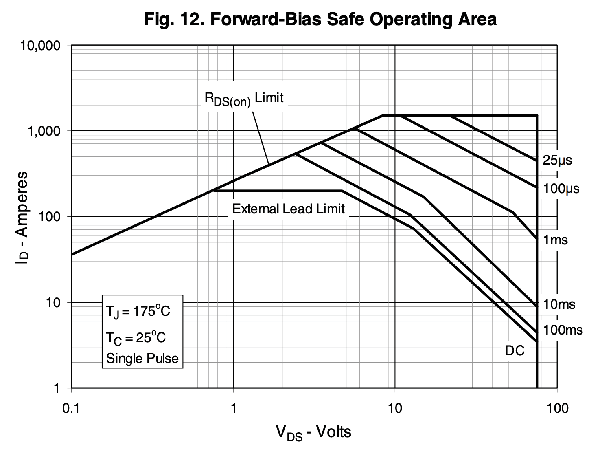
\includegraphics[]{Figures/AppendixA/transistor_specs.pdf}
\caption[Safe operation regime of a MOSFET]{Safe operation regime of the \noted{IXFN 520N075T2} MOSFET. Even though they are in principle rated for up to $\unit[480]{A}$ the maximum safe current is greatly reduced at larger drain to source voltages $V_{DS}$. A high $V_{DS}$ is desirable to reduce the inductive kickback during turn on.}
\label{fig:transistor_specs}
\end{center}
\end{figure*}

{\bf Hand made in vacuum shutters:} Before going into the Zeeman slower, the atoms that were heated in the Rb oven travel to the main oven chamber that is pictured in Figure~\ref{fig:RbLi}b containing a cold-cup and an oven shutter. The cold-cup is a cylindrical shaped copper piece that is attached to the cold end of a thermo-electric cooler (TEC) via a copper rod. We keep the cold-cup temperature at $-\unit[30]{C}$ in order to capture excess Rb atoms in the chamber and prevent damaging the ion pumps. The oven shutter allows us to block or enable the atomic beam. We use a homemade device, made from a re-purposed hard drive disk shutter with a metallic flag attached to its end. The shutter is electrically connected to en electric feedthrough with vacuum-compatible Kapton sealed wires. Other apparatus within the JQI~\cite{BrownThesis,Karina2012} have commercial shutters from \noted{Uniblitz} and some of them have failed in the past. Overall we have found this setup to be very reliable. The only problem we experienced once was some accumulation of Rb on the cold cup that started blocking the atomic beam. To remedy this we reversed the polarity of the TEC and heated the cold cup barely enough so that the accumulated Rb atoms melted and moved away from the aperture of the atomic beam. 

\begin{figure*}[htb]
\begin{center}
\includegraphics[]{Figures/AppendixA/oven_chamber.pdf}
\caption[The RbLi vacuum system]{$\Rb87$ level structure (not to scale). {\bf a.} Ground and first excited state electronic configuration of $\Rb87$ given by the $\{n,\mathbf{L}\}$ quantum numbers. {\bf b.} The interaction between the orbital angular momentum and the spin of the electron leads to the fine splitting of orbitals with $L>0$. The splitting of the $5^2P$ line gives rise to the D1 and D2 lines. {\bf c.} The interaction between the total angular momentum and the nuclear spin causes the fine structure levels to split further into states characterized by the quantum number $F$.}
\label{fig:RbLi}
\end{center}
\end{figure*}

{\bf Ultraviolet LEDs:} We have two $\unit[3]{W}$ ultraviolet LEDs from \noted{Mightex} placed at the glass cell side of the vacuum system. One is aimed at the vacuum window where the slower beam enters and the other is placed aiming at the glass cell. The LEDs prevent Rubidium from depositing on the vacuum system and can conveniently be turned on and off with a TTL signal from the computer. We have found that routinely turning them on (for example, leaving them on overnight) leads to a smoother operation of the system. 

{\bf Mirror mounts with picomotor actuators:} We use \noted{8816-6} picomotor optical mounts from \noted{New Focus Optics} whose deflection angle can be electronically adjusted on the order of microradians. The addition of picomotor mounts has made alignment of laser beams to the atoms significantly easier. We use this mounts on the last tunable mirror before the atoms for beam paths whose alignment is critical, for example in optical dipole trap and Raman beams. 

{\bf Stable polarization of MOT beams:} The light of our MOT beams is coupled to polarization maintaining optical fibers. We found that besides our best efforts to align the polarization of the incoming light to the axis of the fiber the fluctuations in the output polarization could cause considerable instabilities in the BEC production. To keep the polarization clean we placed polarizers at the output of the fibers. We found that despite the power hit we can get from the changes in polarization, this solution leads to a much more stable production of BECs. 

{\bf Lab couch:} When the experiment is functional enough that data can be taken long hours in the lab are often required. When it gets late, the lab couch allows the person running the experiment to take small breaks while experimental 

{\bf Others already mentioned in the main text:} The new master laser from Vescent photonics has been very stable and reliable. The new Mako camera has been very helpful to get rid of unwanted fringes in absorption images. Labscript makes writing experimental sequences very straightforward. 

% mica capacitors for high power RF impedance matching?

\section{The bad}

{\bf Free space dipole laser:} The laser system providing $\unit[1064]{nm}$ light for the optical dipole trap is not fiber coupled and is setup in the same optical table as the vacuum system; we are not able to change the laser without destroying the alignment of the beam with the atoms.  This issue became important while setting up a 1D optical lattice by retro-reflecting one of the dipole trap beams we noticed that the laser mode is not very stable, leading to big fluctuations in the optical lattice. In the original design of the laser system high-power photonic crystal fibers were included but they did not have built in mode expanders which resulted in the tip of the fiber inevitably getting burnt after some time of use. In short, mode expanders are recommended in applications involving large optical powers.

{\bf Water cooling shared between two labs:} The quadrupole and Zeeman slower coils as well as the transistor banks require water cooling due to Joule heating. Our lab space is shared with a Rubidium-Ytterbium ultracold mixtures apparatus~\cite{HeroldThesis} and amongst the things we shared is the water cooling system. The schematic in Figure~\ref{fig:water_cooling} illustrates the layout of the water cooling system. The water was filtered at two different points, first at each line has a $\unit[440]{\mu m}$ particulate filter from \noted{Swagelok} and then the water returning to the heat exchanger is filtered with a low-impedance cellulose cartridge (\noted{McMaster 7191K11}). Both filters only capture impurities in the water for one given flow direction. One of the failure modes which occurs when one of the booster pumps is turned on before the heat exchanger, causing water to flow from one experiment to the other and bringing a collection of nasty things that escapes the filters into the coils. Over the years our system has suffered of clogged filters, clogged coils and broken booster pumps. For best operation it is highly recommended that the cartridge filter is changed and that the Swagelok filters be cleanded at least once a year and that a $10\%$ solution of an anti-corrosive \noted{Optishield Plus} in water is used as a coolant. Even when following this practices, we managed to find lots of gunk and unidentified objects (sand? glass? mud? oxide? dead bacteria?) in the water, just at a slower rate.

\begin{figure*}[htb]
\begin{center}
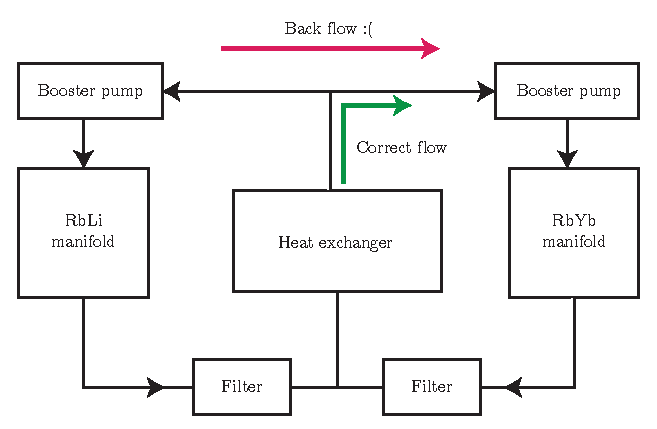
\includegraphics[]{Figures/Chapter4/water_cooling.pdf}
\caption[Water cooling manifold schematic]{Simplified schematic of the shared water cooling manifold.}
\label{fig:water_cooling}
\end{center}
\end{figure*}

\section{The ugly}
The ugly elements are not quite bad but they don't function flawlessly either. If given the option to replace them with something better I definitely would. 

kepcos
BoosTA
too many NI usb devices on the same computer


 
		% %Appendix -- January 2015
\appendix
\renewcommand{\thechapter}{B}
\renewcommand{\chaptername}{Appendix}

\chapter{RbLi: the good, the bad and the ugly}
\label{app:RbLi}

\begin{figure*}[htb]
\begin{center}
\includegraphics[]{Figures/Chapter8/topological_eigenvecs.pdf}
\caption{{\bfseries a} Probabilities as a function of quasimomentum for the three output ports of the interferometer at $t_{\rm free}=\unit[160]{\mu s}$ {\bfseries b} Probabilities as a function of free evolution time $t_{\mathrm{free}}$ for an input state with quasimomentum $(q_1, q_2)=(0.55,-0.92)\,k_{\rm L}$ indicated by the blue star on {\bfseries a} and in the topological ground branch ($n=1$)}
\label{fig:topological_eigenvecs}
\end{center}
\end{figure*}

\begin{figure*}[htb]
\begin{center}
\includegraphics[]{Figures/Chapter8/nontopological_eigenvecs.pdf}
\caption{{\bfseries a} Probabilities as a function of quasimomentum for the three output ports of the interferometer at $t_{\rm free}=\unit[160]{\mu s}$ {\bfseries b} Probabilities as a function of free evolution time $t_{\mathrm{free}}$ for an input state with quasimomentum $(q_1, q_2)=(0.55,-0.92)\,k_{\rm L}$ indicated by the blue star on {\bfseries a} and in the topological ground branch ($n=1$)}
\label{fig:nontopological_eigenvecs}
\end{center}
\end{figure*}


\section{Water cooling stuff}
\section{Electrical installation}
\section{New Rb `oven'}


		%Appendix 
\appendix
\renewcommand{\thechapter}{C}
\renewcommand{\chaptername}{Appendix}

\chapter{New Apparatus}
\label{app:Basement_lab}


	\end{chapter_env}

	\begin{bib_env}
		%\begin{thebibliography}{99}
\setlength{\parskip}{1em}

\newpage 
\bibliographystyle{unsrt}
\bibliography{RFClockStates.bib,MolmerSorensen.bib,Rashba.bib}

%\end{thebibliography}


		% When using Bibtex switch to:
		% \newpage
		% \bibliographystyle{unsrt} 
		% \bibliography{bib_file_1, bib_file_2, ...}
	\end{bib_env}
	
\end{document}
